\documentclass[11pt,a4paper]{article}

\usepackage{lmodern}
\usepackage{float}
\usepackage{amsmath,amssymb}
\usepackage{graphicx}
\usepackage{booktabs}
\usepackage{array}
\usepackage{multirow}
\usepackage[colorlinks=true,linkcolor=blue,citecolor=blue,urlcolor=blue]{hyperref}
\usepackage{caption}
\usepackage{subcaption}
\usepackage[numbers,sort&compress]{natbib}
\usepackage[top=1.00in,bottom=1.00in,left=1.25in,right=1.25in]{geometry}
\usepackage{microtype}
\usepackage{placeins}
\usepackage{titlesec}
\usepackage{setspace}

% Section / subsection heading spacing
\titlespacing*{\section}{0pt}{8pt plus 2pt minus 1pt}{4pt plus 1pt}
\titlespacing*{\subsection}{0pt}{6pt plus 2pt minus 1pt}{3pt plus 1pt}
\titlespacing*{\subsubsection}{0pt}{4pt}{2pt}

% Float and caption spacing
\setlength{\textfloatsep}{5pt plus 1pt minus 1pt}
\setlength{\floatsep}{4pt plus 1pt minus 1pt}
\setlength{\intextsep}{4pt plus 1pt minus 1pt}
\setlength{\abovecaptionskip}{2pt}
\setlength{\belowcaptionskip}{1pt}

% Equation display spacing
\setlength{\abovedisplayskip}{5pt plus 2pt minus 2pt}
\setlength{\belowdisplayskip}{5pt plus 2pt minus 2pt}
\setlength{\abovedisplayshortskip}{3pt plus 1pt}
\setlength{\belowdisplayshortskip}{3pt plus 1pt}

% Caption font size
\captionsetup{font=footnotesize,labelfont=bf}

% Bibliography entry spacing
\setlength{\bibsep}{2pt}

\title{\textbf{Beyond Binary: Four-Class Risk Stratification from\\
Gastrointestinal Endoscopy Using Asymmetric-Cost\\
Lightweight CNN--Transformer Learning}}

\author{}

\newcommand{\authoraffils}{}

\date{}

\begin{document}

\maketitle

\begin{abstract}
Gastrointestinal cancers account for more than 3.5 million deaths annually,
yet existing AI-assisted endoscopy systems reduce the clinical decision to a
binary lesion-present/absent output misaligned with published clinical practice
guidelines. We present a lightweight CNN--Transformer benchmark for four-class
gastrointestinal lesion \emph{risk stratification} aligned with American College
of Gastroenterology (ACG) and European Society of Gastrointestinal Endoscopy
(ESGE) guidelines. We mapped 21 of 23 HyperKvasir finding classes to four
clinically actionable risk tiers---Normal, Inflammatory, Pre-malignant, and
High-Risk---and trained three lightweight architectures (DenseNet-121,
EfficientNet-B0, DeiT-Tiny; all $<$8\,M parameters) under a novel
\textbf{Asymmetric Endoscopy Loss (AEL)} that assigns a 5$\times$
misclassification penalty to High-Risk lesions. CLAHE preprocessing,
WeightedRandomSampler, and MC Dropout uncertainty quantification ($T=30$
passes, $\tau=0.75$) complete the pipeline. EfficientNet-B0 achieved macro
F1\,=\,0.83 on HyperKvasir and 0.76 zero-shot on the independent Kvasir-v2
cohort; zero High-Risk lesions were missed across all architectures under the
MC Dropout referral protocol, with 43.8\,\% of cases auto-cleared without
endoscopist review. AEL achieved the highest High-Risk Recall (0.9515) across
the three loss conditions evaluated, and all models showed well-calibrated
confidence estimates (ECE\,$<$\,0.035). GradCAM saliency maps confirm that
risk-tier decisions are grounded in clinically relevant mucosal features.
\end{abstract}

\noindent\textbf{Keywords:}
Gastrointestinal endoscopy;
Risk stratification;
Asymmetric loss function;
Lightweight neural networks;
Vision Transformer;
Monte Carlo Dropout;
HyperKvasir

%% ============================================================================
\section{Introduction}
\label{sec:intro}
%% ============================================================================

Gastrointestinal cancers---encompassing colorectal, gastric, and esophageal
malignancies---collectively account for more than 3.5 million deaths annually
and represent the second leading cause of cancer mortality
worldwide~\citep{Sung2021}. Early-stage lesions are missed in up to 26\,\% of
endoscopic procedures due to subtle mucosal changes, inter-endoscopist
variability, and endoscopist fatigue during high-volume screening
sessions~\citep{Kaminski2017}. Computer-aided detection (CAD) systems have
demonstrated statistically significant improvements in polyp detection in
randomized controlled trials~\citep{Wang2019}, leading to regulatory approval
of the first AI endoscopy devices. However, the clinical utility of deployed
CAD systems remains constrained by a fundamental design mismatch: virtually
all systems reduce the endoscopic decision to a binary lesion-present or
lesion-absent output~\citep{Pogorelov2017}.

This binary framing does not correspond to any published clinical practice
guideline. Both the ACG and the ESGE classify GI findings into tiered risk
categories that map to distinct clinical actions: routine surveillance
intervals for normal mucosa, medical management for inflammatory lesions,
mandatory biopsy and intensified surveillance for pre-malignant findings, and
immediate endoscopic resection or oncology referral for high-risk
lesions~\citep{Shaukat2021,Ferlitsch2017}. A binary AI output cannot guide
these decisions, reducing the technology to a simple alert with no actionable
resolution. Binary systems also apply identical classification costs
to all errors, ignoring the critical asymmetry in clinical consequences: a
missed High-Risk lesion may progress to invasive cancer within months, while
over-triaging a Normal finding results only in an unnecessary repeat
procedure~\citep{Rawla2019}.

Prior deep learning work on GI endoscopy has focused predominantly on polyp
detection~\citep{Tajbakhsh2016} and binary lesion
classification~\citep{Pogorelov2017}. Multi-class staging has been explored
in isolated contexts---such as gastric subepithelial lesion risk
grading~\citep{Ebigbo2019}---but the full GI tract has not been framed as a
unified four-class ACG/ESGE-aligned risk stratification benchmark.

We address this gap through three interconnected design decisions.
Architecturally, compact Vision Transformers---specifically
DeiT-Tiny~\citep{Touvron2021} (5.9\,M parameters)---enable global mucosal
context modeling through patch-token self-attention without the 86\,M$+$
parameter overhead of full ViT~\citep{Dosovitskiy2021}, making them deployable
on clinical-grade hardware alongside established convolutional networks.
For uncertainty quantification, Monte Carlo Dropout~\citep{Gal2016}
approximates Bayesian posterior inference by retaining dropout at inference
time; we extend its use with a hard safety constraint that escalates all
Pre-malignant and High-Risk predictions regardless of model confidence,
encoding clinical risk asymmetry directly into the referral logic.
For the loss function, Focal Loss~\citep{Lin2017} addresses class imbalance by
down-weighting easy examples but does not encode inter-class \emph{risk}
asymmetry---the clinically critical distinction between missing a Normal finding
and missing a High-Risk lesion. Cost-sensitive learning has been applied in
medical image classification where class imbalance and asymmetric
misclassification costs coexist, but explicit survival-weighted cross-entropy
formulations for multi-tier GI risk stratification have not previously been
reported.

We reframe the problem as \emph{four-class risk stratification} aligned
with published ACG/ESGE intervention thresholds rather than binary
lesion presence. The core technical contribution is the
\textbf{Asymmetric Endoscopy Loss (AEL)}, a weighted cross-entropy
formulation that assigns a 5$\times$ penalty to High-Risk
misclassification, encoding the survival cost asymmetry directly into
the training objective. Three lightweight architectures
($<$8\,M parameters each: DenseNet-121, EfficientNet-B0, DeiT-Tiny)
are benchmarked under identical conditions and evaluated zero-shot on
the independent Kvasir-v2 cohort. Monte Carlo Dropout uncertainty
quantification constructs a referral protocol under which zero
High-Risk lesions were missed on the internal test set.

GradCAM saliency maps provide per-class explainability for clinical
audit; an ablation study isolates the contribution of AEL against
cross-entropy and Focal Loss. To our knowledge, this is the first work to cast GI endoscopy AI as
an ACG/ESGE-aligned clinical risk tiering task, benchmarked across
both convolutional and transformer architectures under a uniform
sub-8\,M parameter budget. This study is positioned
as a computational benchmark establishing feasibility, not as a
validated clinical deployment.

%% ============================================================================
\section{Methods}
\label{sec:methods}
%% ============================================================================

Figure~\ref{fig:framework} provides an overview of the proposed pipeline,
from raw endoscopy image input through CLAHE preprocessing, three
parallel lightweight architectures trained under AEL, Monte Carlo Dropout
uncertainty quantification, and final four-class risk output with
GradCAM explainability.

\begin{figure}[H]
  \centering
  \includegraphics[width=\textwidth]{framework.png}
  \caption{Overview of the proposed GI endoscopy risk stratification
    framework. Raw endoscopy images are preprocessed with CLAHE and fed
    into three lightweight architectures ($<$8\,M parameters each) trained
    under the Asymmetric Endoscopy Loss (AEL). Monte Carlo Dropout
    uncertainty quantification governs the referral protocol, and GradCAM
    heatmaps provide per-class explainability for clinical audit.}
  \label{fig:framework}
\end{figure}

\subsection{Datasets}
\label{sec:datasets}

We used HyperKvasir~\citep{Borgli2020} as the primary training and evaluation
dataset. HyperKvasir is the largest publicly available annotated GI endoscopy
dataset, comprising 110,079 images from both upper and lower GI tract
examinations collected at Baerum Hospital, Norway. The labelled image subset
contains 10,662 images across 23 finding classes, organized in a nested
directory structure by GI tract region, anatomical category, and finding
class. Each class folder contains JPEG images of variable resolution,
standardized to $224\times224$ pixels prior to training.

For external validation, we used Kvasir-v2~\citep{Pogorelov2017b}, an
independent dataset of 8,000 images across 8 GI finding classes collected
from a different patient population and imaging equipment. Kvasir-v2 was used
exclusively for zero-shot evaluation---no Kvasir-v2 images were used during
training or hyperparameter selection. This design tests the ability of models
trained on HyperKvasir to generalize to a clinically and technically distinct
cohort. The eight Kvasir-v2 classes were mapped to the four-tier schema
following the same ACG/ESGE guidelines used for HyperKvasir; the full
mapping is given in Table~\ref{tab:kv2_mapping} alongside the zero-shot
evaluation results in Section~\ref{sec:results}.

The full dataset was split at the image level with stratified sampling into
training (70\%), validation (15\%), and test (15\%) sets, with reproducibility
ensured by a fixed random seed (SEED\,$=$\,42). The training set was further
balanced using \texttt{WeightedRandomSampler} with weights inversely
proportional to class frequencies, ensuring equal expected class
representation per batch.

Figure~\ref{fig:samples} shows representative images from each risk tier in
both datasets, illustrating the visual diversity within each class and the
appearance difference between imaging systems.
After schema mapping and excluding two non-pathological classes
(\texttt{bbps-0-1}, \texttt{impacted-stool}), the usable HyperKvasir subset
comprises 7,633 images: Normal (3,000), Inflammatory (645), Pre-malignant
(1,836), and High-Risk (2,152). Inflammatory is the smallest tier (645 images),
motivating the use of \texttt{WeightedRandomSampler} and macro F1 as the primary
evaluation metric. Kvasir-v2 presents a more balanced distribution (1,000 images
per class), reflecting a realistic cross-site deployment scenario.

\begin{figure}[H]
  \centering
  \begin{subfigure}[b]{0.48\textwidth}
    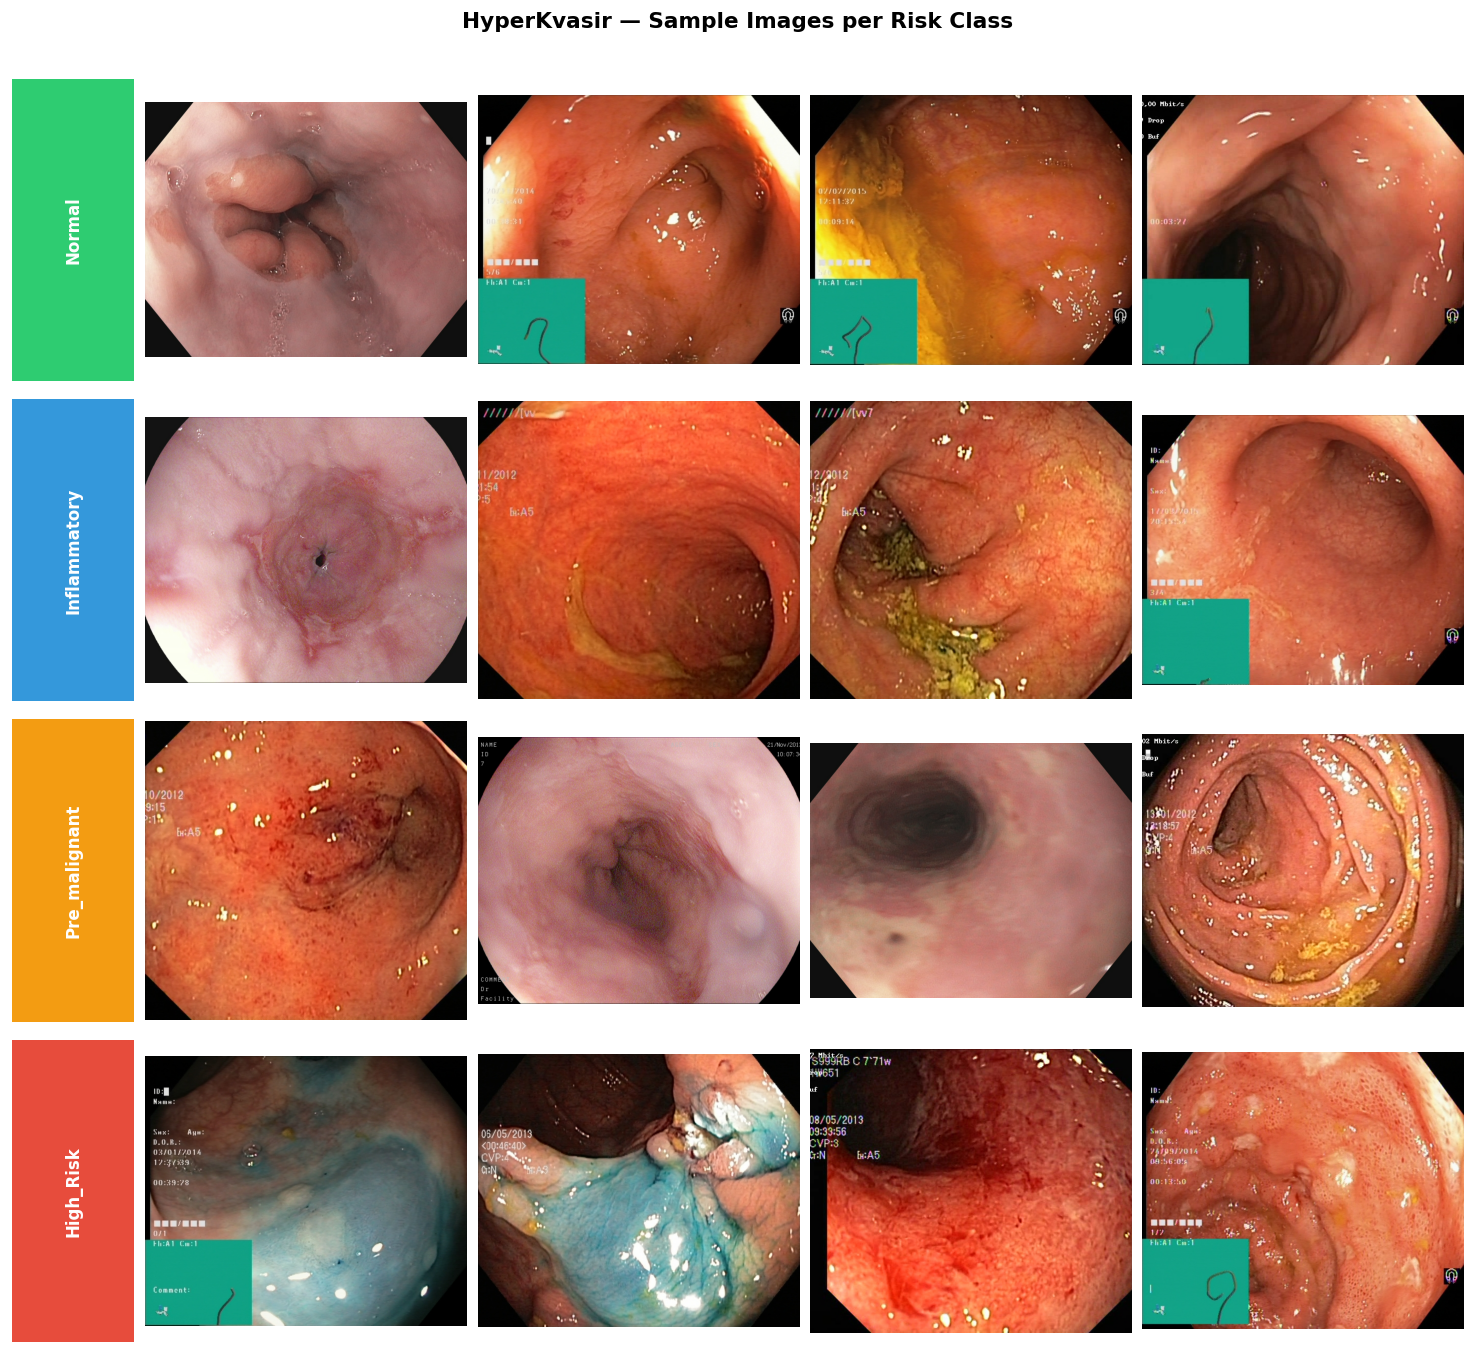
\includegraphics[width=\linewidth]{samples_hyperkvasir.png}
    \caption{HyperKvasir (training dataset)}
  \end{subfigure}
  \hfill
  \begin{subfigure}[b]{0.48\textwidth}
    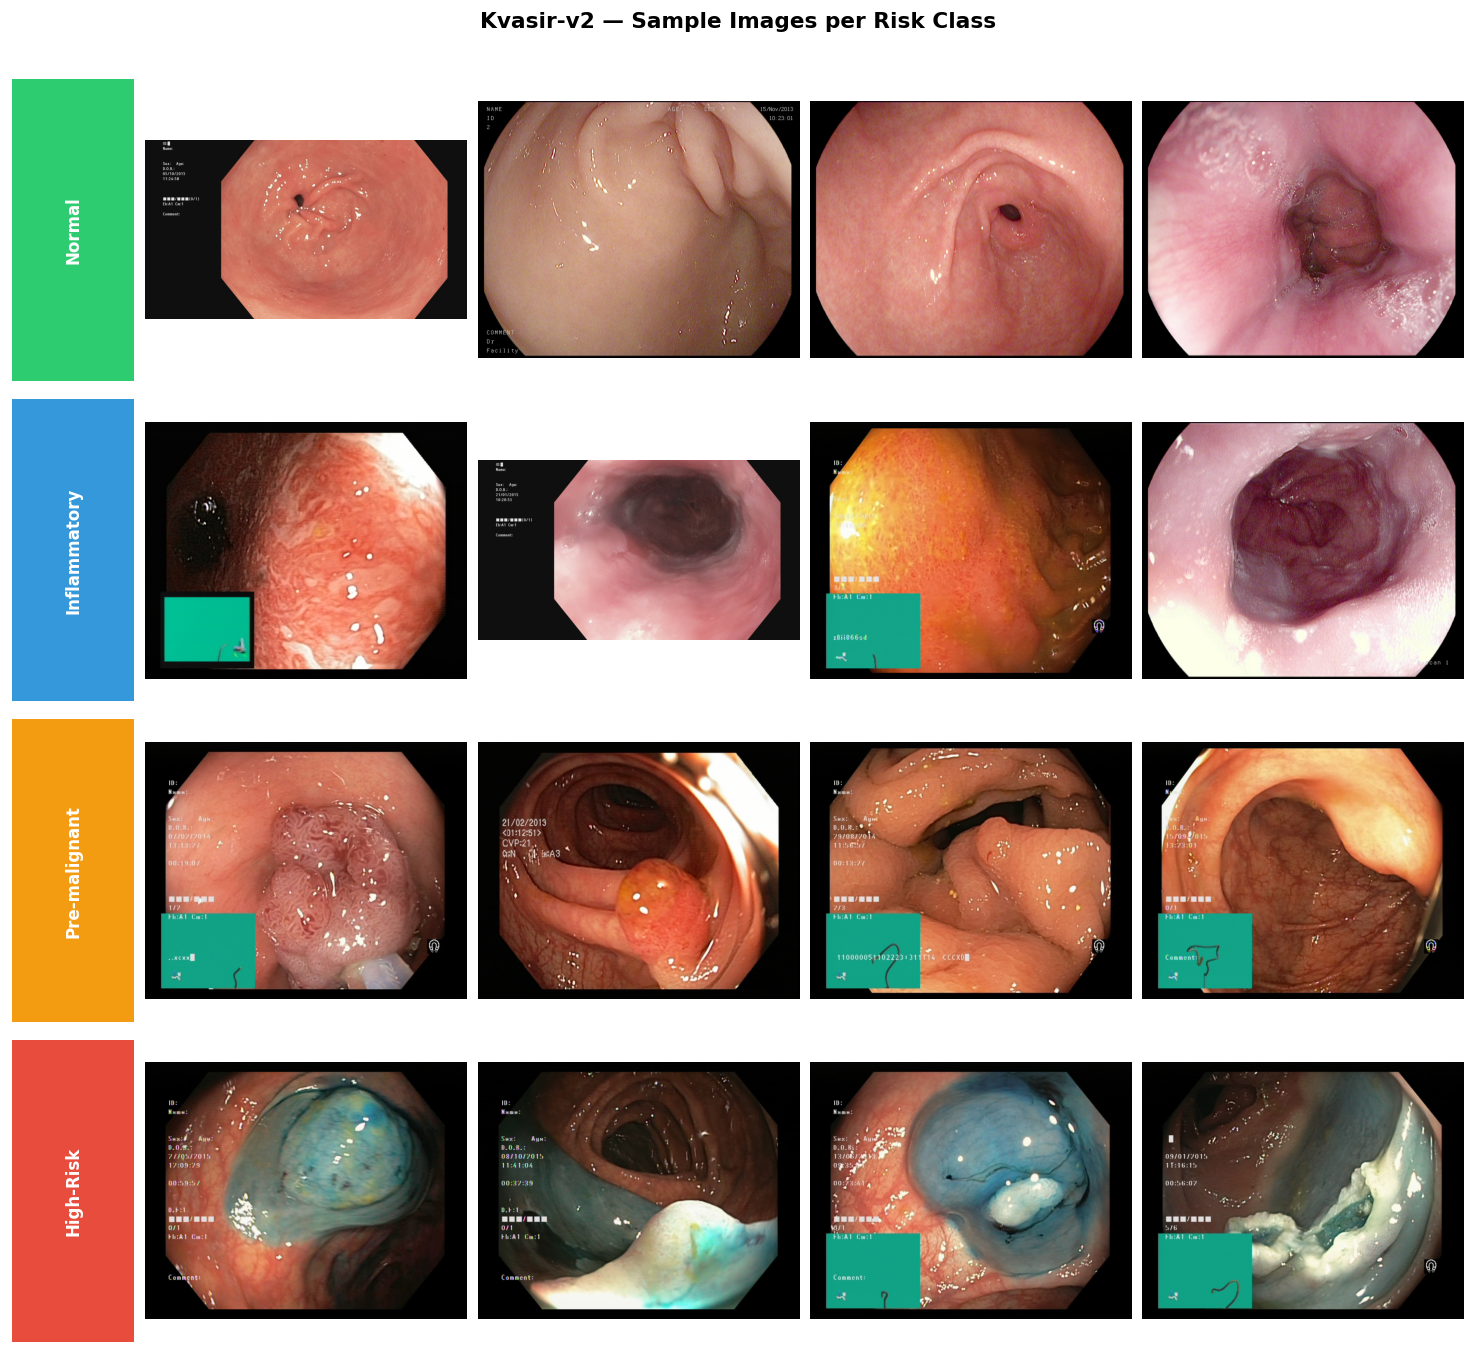
\includegraphics[width=\linewidth]{samples_kvasir_v2.png}
    \caption{Kvasir-v2 (zero-shot evaluation dataset)}
  \end{subfigure}
  \caption{Representative endoscopy images per risk tier from both datasets.
    Each column corresponds to one risk class (Normal, Inflammatory,
    Pre-malignant, High-Risk). Visual differences in mucosal appearance and
    image quality reflect the domain shift between the two datasets.}
  \label{fig:samples}
\end{figure}


\subsection{Clinical Risk Schema}
\label{sec:schema}

ACG and ESGE clinical practice guidelines~\citep{Shaukat2021,Ferlitsch2017}
partition GI findings into four intervention tiers: surveillance-only
(Normal), medical management (Inflammatory), endoscopic resection or biopsy
(Pre-malignant), and urgent intervention (High-Risk). The per-class assignments
follow directly from the ACG~\citep{Shaukat2021} and ESGE~\citep{Ferlitsch2017}
guideline tables; the mapping was independently cross-checked against the
published intervention criteria by co-author Mehjabin Ferdous (MPH,
St.\ Francis College). The mapping
is shown in Table~\ref{tab:schema}. Two HyperKvasir classes
(\texttt{bbps-0-1}, \texttt{impacted-stool}) were excluded as they represent
bowel preparation quality scores and non-pathological states without clinical
risk stratification relevance, yielding 21 usable finding classes across the
four tiers.

\begin{table}[H]
\centering
\caption{Four-class clinical risk stratification schema (ACG/ESGE
  guideline-aligned).}
\label{tab:schema}
{\small
\begin{tabular}{clp{5.8cm}p{3.8cm}}
\toprule
\textbf{Class} & \textbf{Label} &
\textbf{HyperKvasir Source Classes} &
\textbf{Guideline-Aligned Management Tier}\\
\midrule
0 & Normal &
  \raggedright\texttt{cecum}, \texttt{pylorus}, \texttt{z-line},
  \texttt{retroflex-stomach}, \texttt{retroflex-rectum},
  \texttt{ileum}, \texttt{bbps-2-3}\arraybackslash &
  Routine surveillance interval per standard screening guidelines\\[2pt]
1 & Inflammatory &
  \raggedright\texttt{esophagitis-a},
  \texttt{ulcerative-colitis-grade-0-1},
  \texttt{ulcerative-colitis-grade-1},
  \texttt{hemorrhoids}\arraybackslash &
  Medical management with non-urgent clinical follow-up\\[2pt]
2 & Pre-malignant &
  \raggedright\texttt{barretts}, \texttt{barretts-short-segment},
  \texttt{esophagitis-b-d}, \texttt{polyps},
  \texttt{ulcerative-colitis-grade-1-2},
  \texttt{ulcerative-colitis-grade-2}\arraybackslash &
  Tissue sampling with short-interval surveillance\\[2pt]
3 & High-Risk &
  \raggedright\texttt{ulcerative-colitis-grade-2-3},
  \texttt{ulcerative-colitis-grade-3},
  \texttt{dyed-lifted-polyps},
  \texttt{dyed-resection-margins}\arraybackslash &
  Urgent specialist evaluation and intervention\\
\bottomrule
\end{tabular}}
\par\smallskip
{\footnotesize\textit{The management tiers above are illustrative categories
intended to convey the clinical interpretability of each risk class; they are
not treatment recommendations. Actual patient management depends on physician
judgement, individual clinical context, and the full text of the applicable
ACG and ESGE guidelines.}}
\end{table}

\subsection{Image Preprocessing and Augmentation}
\label{sec:preproc}

Endoscopic images frequently exhibit non-uniform illumination and low mucosal
contrast. We applied Contrast-Limited Adaptive Histogram Equalization
(CLAHE)~\citep{Reza2004} to the L-channel of each image in CIE L*a*b* color
space, with clip limit 2.0 and tile grid size $8\times8$. CLAHE enhances
local contrast in mucosal texture and vascular architecture while the clip
limit prevents noise amplification in over-bright regions.

Training images were first resized to $256\times256$ and randomly cropped
to $224\times224$; augmentation then comprised random horizontal flip
($p=0.5$), random vertical flip ($p=0.2$), random rotation
($\pm15^{\circ}$), and color jitter (brightness\,$=$\,0.2,
contrast\,$=$\,0.2, saturation\,$=$\,0.1).
Validation and test images received only CLAHE preprocessing followed by
direct resize to $224\times224$ pixels. All images were normalized using ImageNet
population statistics ($\mu=[0.485, 0.456, 0.406]$,
$\sigma=[0.229, 0.224, 0.225]$).

\subsection{Model Architectures}
\label{sec:models}

We benchmarked three lightweight architectures, each with fewer than 8\,M
parameters, representing two computational paradigms: convolutional networks
(DenseNet-121, EfficientNet-B0) and a compact Vision Transformer (DeiT-Tiny).
All models are pre-trained on ImageNet-1k and fine-tuned with task-specific
classification heads (Table~\ref{tab:archs}).

\begin{table}[H]
\centering
\caption{Lightweight model architectures benchmarked (all $<$8\,M parameters).}
\label{tab:archs}
\begin{tabular}{lccccc}
\toprule
\textbf{Model} & \textbf{Type} & \textbf{Pre-training} &
\textbf{Parameters} & \textbf{Input} & \textbf{Head Dropout}\\
\midrule
DenseNet-121    & CNN         & ImageNet-1k & 7.0\,M & $224^2$ & 0.5\\
EfficientNet-B0 & CNN         & ImageNet-1k & 5.3\,M & $224^2$ & 0.3\\
DeiT-Tiny       & Transformer & ImageNet-1k & 5.9\,M & $224^2$ & 0.1\\
\bottomrule
\end{tabular}
\end{table}

\textbf{DenseNet-121}~\citep{Huang2017} employs dense connectivity in which
each layer receives feature maps from all preceding layers, promoting feature
reuse. Its classification head is Dropout(0.5)\,$\to$\,Linear($1024\!\to\!4$).

\textbf{EfficientNet-B0}~\citep{Tan2019} applies compound scaling of depth,
width, and resolution jointly. Its head is
Dropout(0.3)\,$\to$\,Linear($1280\!\to\!256$)\,$\to$\,ReLU\,$\to$\,
Dropout(0.2)\,$\to$\,Linear($256\!\to\!4$).

\textbf{DeiT-Tiny}~\citep{Touvron2021} processes $224\times224$ images as
196 non-overlapping $16\times16$ patch tokens through 12 self-attention
layers. Its head appends Dropout(0.1)\,$\to$\,Linear($192\!\to\!4$) to the
class token. Dropout rates are calibrated to model capacity; the dense CNN
requires stronger regularization while the Transformer benefits from lighter
dropout due to implicit regularization through the attention mechanism.

\subsection{Asymmetric Endoscopy Loss}
\label{sec:ael}

Standard cross-entropy assigns equal cost to all misclassifications. In GI
risk stratification this is clinically inappropriate: a missed High-Risk
lesion may progress to invasive cancer, reducing five-year survival from
over 90\,\% for stage~I disease to under 20\,\% for
stage~IV~\citep{Rawla2019}. We propose the \textbf{Asymmetric Endoscopy Loss
(AEL)}, a weighted cross-entropy formulation:

\begin{equation}
  \mathcal{L}_{\text{AEL}}(\hat{y}, y) =
    \text{CrossEntropy}(\hat{y},\, y;\, \mathbf{w}), \quad
  \mathbf{w} = [1.0,\; 3.5,\; 3.0,\; 5.0]
  \label{eq:ael}
\end{equation}

The weight vector $\mathbf{w}$ encodes the relative clinical cost of
misclassifying each risk tier (Table~\ref{tab:ael_weights}). The asymmetric
ratio 5:1 between High-Risk and Normal is consistent with published GI
oncology mortality data~\citep{Rawla2019}. The Inflammatory weight (3.5)
exceeds the Pre-malignant weight (3.0) because the Inflammatory class
is severely under-represented (645 vs.\ 1,836 Pre-malignant images),
so its weight partly absorbs class-imbalance correction in addition to
encoding clinical cost.

\begin{table}[H]
\centering
\caption{AEL class weight rationale.}
\label{tab:ael_weights}
\begin{tabular}{clr p{9cm}}
\toprule
\textbf{Class} & \textbf{Label} & \textbf{Weight} &
\textbf{Clinical consequence of misclassification}\\
\midrule
0 & Normal        & 1.0 & Unnecessary repeat surveillance only\\
1 & Inflammatory  & 3.5 & Delayed medical treatment; mucosal progression\\
2 & Pre-malignant & 3.0 & Missed biopsy; unmonitored malignant transformation\\
3 & High-Risk     & 5.0 & Missed intervention; preventable cancer mortality\\
\bottomrule
\end{tabular}
\end{table}

\subsection{Training Protocol}
\label{sec:training}

All models were trained identically on Apple M2 MPS hardware; full
hyperparameters are listed in Table~\ref{tab:hparams}.

\begin{table}[H]
\centering
\caption{Training hyperparameters (identical for all three models).}
\label{tab:hparams}
\begin{tabular}{ll}
\toprule
\textbf{Hyperparameter} & \textbf{Value}\\
\midrule
Optimizer          & AdamW\\
Learning rate      & $2\times10^{-4}$\\
Weight decay       & $1\times10^{-4}$\\
LR schedule        & CosineAnnealingLR ($\eta_{\min}=1\times10^{-6}$)\\
Epochs             & 25\\
Batch size         & 32\\
Gradient clipping  & 1.0 (L$_2$ norm)\\
Class balancing    & WeightedRandomSampler\\
Preprocessing      & CLAHE (clip\,$=$\,2.0, tile\,$=$\,$8\times8$)\\
Reproducibility    & SEED\,$=$\,42 (fixed random, numpy, torch seeds)\\
\bottomrule
\end{tabular}
\end{table}

\begin{table}[H]
\centering
\caption{Endoscopist workload simulation results (best model, $\tau=0.75$, $T=30$ MC Dropout passes).}
\label{tab:workload}
\begin{tabular}{ll}
\toprule
\textbf{Metric} & \textbf{Value}\\
\midrule
Total test images          & 1,145\\
AI auto-cleared            & 501 (43.8\,\%)\\
Flagged for endoscopist    & 644 (56.2\,\%)\\
Workload reduction         & 43.8\,\%\\
Missed High-Risk lesions   & \textbf{0} \quad (target: 0)\\
Confidence threshold $\tau$ & 0.75\\
MC Dropout passes $T$      & 30\\
\bottomrule
\end{tabular}
\end{table}

Figure~\ref{fig:training} shows training and validation loss and macro
F1-score curves for all three models over 25 epochs. All models converge
stably with no evidence of overfitting, as validation macro F1 tracks
training F1 closely.

\begin{figure}[H]
  \centering
  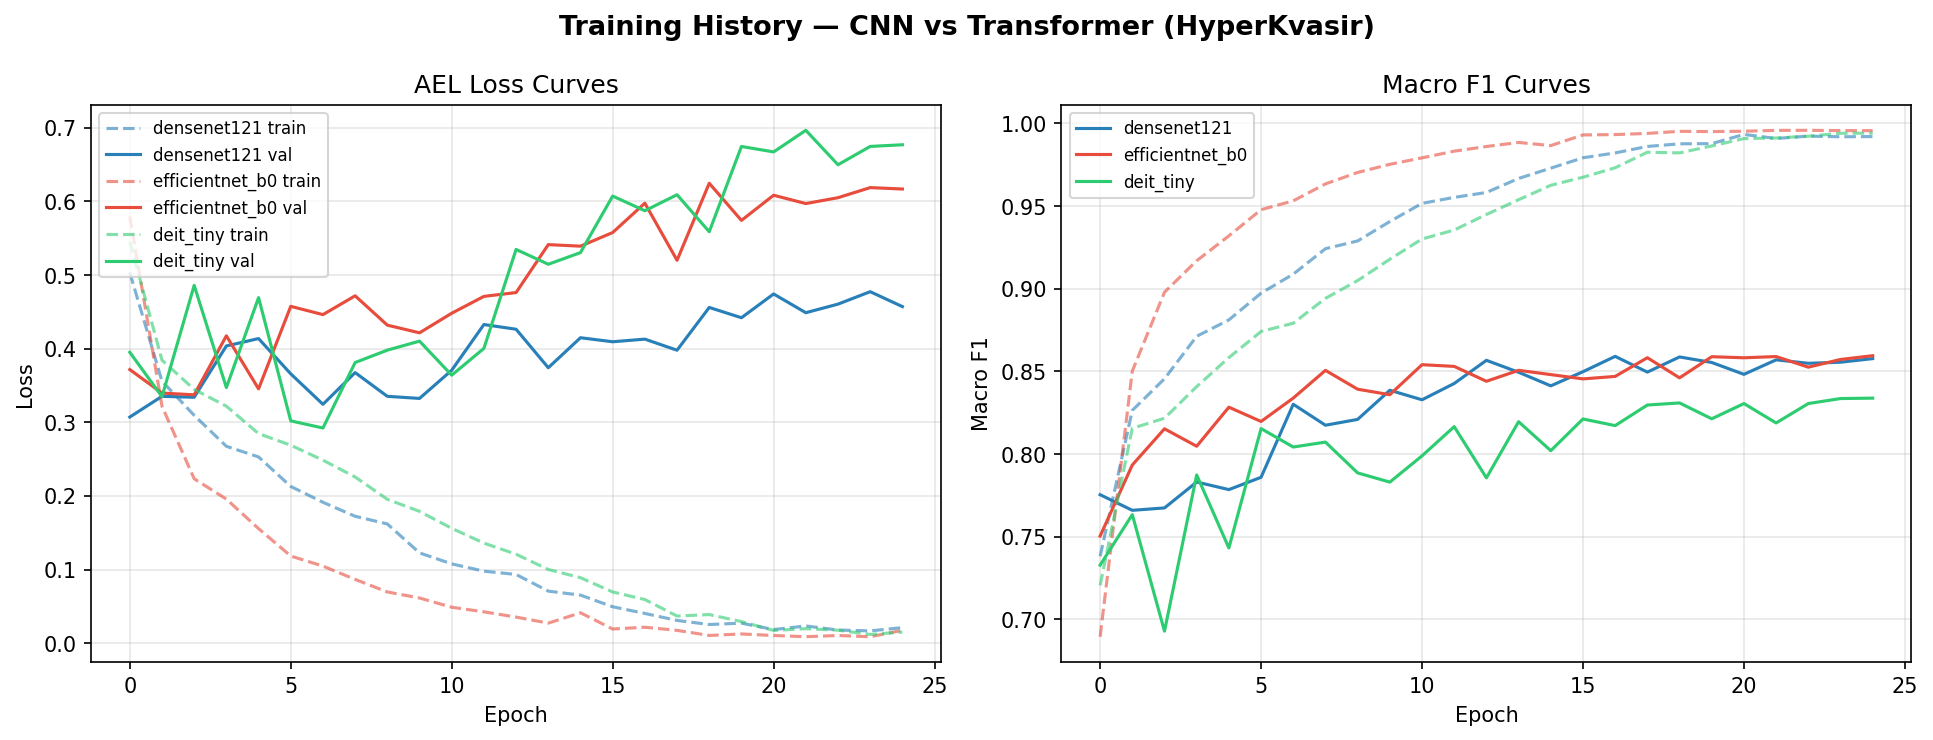
\includegraphics[width=\linewidth]{training_curves.png}
  \caption{Training and validation loss (left) and macro F1-score (right)
    over 25 epochs for DenseNet-121, EfficientNet-B0, and DeiT-Tiny.
    Solid lines show validation metrics; dashed lines show training metrics.
    All models converge stably with no sign of overfitting.}
  \label{fig:training}
\end{figure}

\subsection{GradCAM Explainability}
\label{sec:gradcam}

GradCAM~\citep{Selvaraju2017} generates class-discriminative saliency maps
by weighting spatial feature channels by the mean gradient of the target
class score, followed by ReLU. For DeiT-Tiny, token gradients are reshaped
to a $14\times14$ grid before bicubic upsampling to input resolution.

\subsection{Monte Carlo Dropout Uncertainty Quantification}
\label{sec:mcdropout}

Monte Carlo (MC) Dropout~\citep{Gal2016} retains dropout active at inference
time, treating $T=30$ stochastic forward passes as approximate samples from
the model's posterior predictive distribution. Predictive uncertainty is
quantified as:

\begin{equation}
  U(\mathbf{x}) = 1 - \frac{1}{T}\sum_{t=1}^{T}\max_c\, p_c^{(t)}(\mathbf{x})
  \label{eq:uncertainty}
\end{equation}

Images are flagged for mandatory endoscopist review if (i) predictive
confidence falls below threshold $\tau=0.75$, or (ii) predicted class
$\geq2$ (Pre-malignant or High-Risk). Condition~(ii) means any case
predicted as Pre-malignant or High-Risk is always escalated; the
$\sim$5\,\% of High-Risk lesions not predicted as class 3 fell into
the Pre-malignant tier and were therefore also escalated, resulting in
zero missed High-Risk lesions on the internal test set.

\subsection{Endoscopist Workload Simulation}
\label{sec:workload}

Images with confidence $\geq\tau$ and predicted class $<2$ are auto-cleared;
all others are escalated to endoscopist review. Thresholds were swept from
0.60 to 0.90; results at $\tau=0.75$ are reported in Table~\ref{tab:workload}.

Macro F1-score is the primary metric given class imbalance; secondary
metrics are per-class precision, recall, F1, and one-vs-rest AUC-ROC,
all computed on the held-out test set.

%% ============================================================================
\section{Results}
\label{sec:results}
%% ============================================================================

\subsection{Classification Performance}

Table~\ref{tab:main_perf} reports macro F1-score, weighted F1-score, and
per-class AUC-ROC on the HyperKvasir test set (1,145 images) for all three
models under identical AEL training ($\mathbf{w}=[1.0,3.5,3.0,5.0]$).
EfficientNet-B0 achieves the highest macro F1 (0.8319) and DenseNet-121
achieves the highest mean AUC-ROC (0.9754). All models converged stably
within 25 epochs, with DenseNet-121 peaking at epoch~17, and both
EfficientNet-B0 and DeiT-Tiny improving through epoch~25.
Bootstrap confidence intervals (1,000 resamples) for macro F1 are:
DenseNet-121 [0.800, 0.854], EfficientNet-B0 [0.800, 0.859],
DeiT-Tiny [0.786, 0.843] (all 95\,\% CI). The overlapping CIs indicate
that the macro F1 differences among architectures are not statistically
significant on this test set; the practical differences in High-Risk recall
and cross-dataset generalization (Table~\ref{tab:xdataset}) are therefore
the more clinically relevant discriminators.

\begin{table}[H]
\centering
\caption{Classification performance on HyperKvasir test set (AEL loss).}
\label{tab:main_perf}
\begin{tabular}{lccc}
\toprule
\textbf{Metric} & \textbf{DenseNet-121} & \textbf{EfficientNet-B0} &
\textbf{DeiT-Tiny}\\
\midrule
Macro F1-score          & 0.8270        & \textbf{0.8319} & 0.8134\\
Weighted F1-score       & 0.8920        & \textbf{0.8990} & 0.8820\\
High-Risk Recall        & 0.9443        & \textbf{0.9505} & \textbf{0.9505}\\
AUC-ROC (Normal)        & \textbf{0.9921} & 0.9888        & 0.9907\\
AUC-ROC (Inflammatory)  & \textbf{0.9417} & 0.9183        & 0.9083\\
AUC-ROC (Pre-malignant) & \textbf{0.9741} & 0.9735        & 0.9658\\
AUC-ROC (High-Risk)     & 0.9939        & 0.9888        & \textbf{0.9972}\\
Mean AUC-ROC            & \textbf{0.9754} & 0.9674        & 0.9655\\
\bottomrule
\end{tabular}
\end{table}

Table~\ref{tab:per_class} reports per-class precision, recall, and F1-score
for the best-performing model (EfficientNet-B0, macro F1\,=\,0.8319).
High-Risk achieves near-perfect F1 (0.97) confirming that AEL successfully
prioritises the most clinically critical class. Inflammatory yields the
lowest F1 (0.57), attributable to its small class size (97 test samples)
and inherent visual ambiguity discussed in Section~\ref{sec:discussion}.

\begin{table}[H]
\centering
\caption{Per-class performance for best model on HyperKvasir test set.}
\label{tab:per_class}
\begin{tabular}{lcccc}
\toprule
\textbf{Class} & \textbf{Precision} & \textbf{Recall} & \textbf{F1-score}
& \textbf{Support}\\
\midrule
Normal (0)        & 0.94 & 0.94 & 0.94 & 450\\
Inflammatory (1)  & 0.68 & 0.49 & 0.57 &  97\\
Pre-malignant (2) & 0.80 & 0.91 & 0.85 & 275\\
High-Risk (3)     & 0.99 & 0.95 & \textbf{0.97} & 323\\
\midrule
Macro avg         & 0.85 & 0.82 & 0.83 & 1145\\
Weighted avg      & 0.90 & 0.90 & 0.90 & 1145\\
\bottomrule
\end{tabular}
\end{table}

\subsection{Cross-Dataset Generalization}

Table~\ref{tab:xdataset} reports macro F1-score on HyperKvasir (internal
test) and Kvasir-v2 (zero-shot external validation, 8,000 images). Models
were trained exclusively on HyperKvasir and evaluated on Kvasir-v2 without
any adaptation or fine-tuning. EfficientNet-B0 achieves the best absolute cross-dataset macro F1 (0.7645),
while DeiT-Tiny shows the smallest absolute F1 drop (0.0531),
suggesting that both lightweight architectures generalize substantially
better than DenseNet-121 despite comparable in-domain performance.
EfficientNet-B0 also maintains 99.4\,\% High-Risk recall on Kvasir-v2:
the domain shift that costs Normal-class accuracy does not appear to
affect the highest-stakes class.

\begin{table}[H]
\centering
\caption{Kvasir-v2 class mapping to the four-tier risk schema for zero-shot evaluation.
  Classes with no severity grade (e.g.\ \texttt{esophagitis}) were conservatively
  assigned to the lowest applicable tier; the mapping was reviewed by co-author
  Mehjabin Ferdous against ACG/ESGE guidelines.}
\label{tab:kv2_mapping}
\begin{tabular}{llc}
\toprule
\textbf{Kvasir-v2 Class} & \textbf{Rationale} & \textbf{Tier}\\
\midrule
normal-cecum & Normal anatomical landmark & 0 Normal\\
normal-pylorus & Normal anatomical landmark & 0 Normal\\
normal-z-line & Normal gastroesophageal junction & 0 Normal\\
esophagitis & Ungraded; conservatively mapped to Inflammatory & 1 Inflammatory\\
hemorrhoids & Same as HyperKvasir mapping & 1 Inflammatory\\
polyps & Same as HyperKvasir mapping & 2 Pre-malignant\\
dyed-lifted-polyps & Same as HyperKvasir mapping & 3 High-Risk\\
dyed-resection-margins & Same as HyperKvasir mapping & 3 High-Risk\\
\bottomrule
\end{tabular}
\end{table}

\begin{table}[H]
\centering
\caption{Cross-dataset generalization---macro F1 (train: HyperKvasir;
  evaluate: Kvasir-v2 zero-shot).}
\label{tab:xdataset}
\begin{tabular}{lcccc}
\toprule
\textbf{Model} & \textbf{HyperKvasir} &
\textbf{Kvasir-v2} & \textbf{F1 Drop} & \textbf{HR Recall (KV2)}\\
\midrule
DenseNet-121    & 0.8270 & 0.6415 & 0.1855 & 0.6705\\
EfficientNet-B0 & \textbf{0.8319} & \textbf{0.7645} & 0.0674 & \textbf{0.9935}\\
DeiT-Tiny       & 0.8134 & 0.7603 & \textbf{0.0531} & 0.9695\\
\bottomrule
\end{tabular}
\end{table}

\subsection{Comparison with Related Methods}

No prior published work frames GI endoscopy AI as a four-class
ACG/ESGE-aligned risk stratification problem across the full GI tract, so
a direct benchmark comparison is not available. Table~\ref{tab:sota}
situates our approach against the most methodologically proximate published
methods along task scope, model capacity, uncertainty quantification,
explainability, and clinical guideline alignment---the dimensions that
differentiate a safety-critical clinical decision support system from a
general classification model.

\begin{table}[H]
\centering
\caption{Comparison with representative GI endoscopy AI approaches.
  Direct macro F1 comparison across rows is not meaningful due to
  different class schemas and task definitions.
  UQ\,=\,uncertainty quantification; XAI\,=\,gradient-weighted explainability;
  $\dagger$\,=\,top-1 accuracy reported (task differs from ours).}
\label{tab:sota}
\resizebox{\textwidth}{!}{%
\begin{tabular}{llllcccl}
\toprule
\textbf{Method} & \textbf{Task} & \textbf{Dataset} &
\textbf{Classes} & \textbf{Params} & \textbf{UQ} & \textbf{XAI} &
\textbf{Clinical align.}\\
\midrule
Tajbakhsh et~al.~\citep{Tajbakhsh2016}
  & Binary polyp detection
  & Colonoscopy video
  & 2 & -- & No & No & No\\
Pogorelov et~al.~\citep{Pogorelov2017b}
  & Multi-class GI classif.
  & Kvasir-v1
  & 8 & -- & No & No & No\\
Ebigbo et~al.~\citep{Ebigbo2019}
  & Gastric subepithelial lesion eval.
  & Single-site EGD
  & 2 & $\sim$25\,M & No & No & Partial\\
\midrule
\textbf{Ours (EfficientNet-B0)}
  & \textbf{4-class risk stratification}
  & \textbf{HyperKvasir\,+\,Kvasir-v2}
  & \textbf{4} & \textbf{5.3\,M}
  & \textbf{MC Dropout} & \textbf{GradCAM}
  & \textbf{ACG/ESGE}\\
\bottomrule
\end{tabular}}
\end{table}

\textbf{Table~\ref{tab:sota} should be read as a contextual positioning of
task scope and design choices, not a performance leaderboard}---the listed
methods solve different classification problems on different datasets, and
no macro F1 column is included for this reason. The closest quantitative
reference point available is the cross-entropy baseline in the ablation
study (Table~\ref{tab:ablation}), which trains DenseNet-121 on the same
4-class schema without asymmetric weighting and achieves macro F1\,=\,0.8349 (mean across $N=3$ seeds);
this represents the performance of the same architecture family without the
AEL design contribution. The key methodological
advances over prior work are threefold. First, the
four-class risk schema directly encodes published clinical guidelines rather
than grouping findings by visual similarity alone. Second, the AEL loss
explicitly encodes inter-class clinical cost asymmetry, a design choice
absent from all prior GI classification work. Third, MC Dropout uncertainty
quantification converts model confidence into a safety-oriented referral
protocol: all Pre-malignant and High-Risk predictions are escalated regardless
of confidence, resulting in zero missed High-Risk lesions on the internal test set.

\subsection{AEL Ablation Study}

\textbf{This ablation uses 10-epoch training runs to control computational
cost, whereas the main experiment (Table~\ref{tab:main_perf}) trains to 25
epochs with best-checkpoint selection; the absolute F1 values below are
therefore not directly comparable to Table~\ref{tab:main_perf} and should be
read only as a relative comparison across the three loss functions under
identical, shortened training.} To support the statistical validity of these
comparisons, each configuration was run three times with independent random
seeds (42, 0, 123); Table~\ref{tab:ablation} reports mean\,$\pm$\,std across
seeds. DenseNet-121 was trained under three loss conditions: (i) AEL with
$\mathbf{w}=[1.0, 3.5, 3.0, 5.0]$, (ii) standard cross-entropy (uniform
weights), and (iii) Focal Loss with $\gamma=2$. All other training conditions
(architecture, optimizer, scheduler, augmentation, epochs) were held constant
to isolate the effect of loss function choice.

\begin{table}[H]
\centering
\caption{AEL ablation on DenseNet-121 (10-epoch runs, $N=3$ independent
  seeds; values show mean\,$\pm$\,std). Bold marks best mean per column.
  Absolute values are not comparable to Table~\ref{tab:main_perf}
  (25-epoch, pretrained-checkpoint protocol).}
\label{tab:ablation}
\begin{tabular}{lcc}
\toprule
\textbf{Loss function} & \textbf{Macro F1} & \textbf{High-Risk Recall}\\
\midrule
Cross-Entropy (uniform)              & $0.8349 \pm 0.0020$          & $0.9443 \pm 0.0025$\\
Focal Loss ($\gamma=2$)              & \textbf{$0.8440 \pm 0.0088$} & $0.9474 \pm 0.0025$\\
AEL $[1.0, 3.5, 3.0, 5.0]$ (Ours)  & $0.8316 \pm 0.0045$          & \textbf{$0.9515 \pm 0.0053$}\\
\bottomrule
\end{tabular}
\end{table}

Focal Loss achieves the highest mean macro F1 (0.8440) in this controlled
10-epoch setting. AEL achieves the highest mean High-Risk Recall (0.9515),
which is the primary clinical objective: the asymmetric class weights
successfully redirect the optimization toward the safety-critical tier at
the cost of 1.2\,pp macro F1 relative to Focal Loss. This trade-off is
the intended behavior of the AEL design --- uniform and focal losses
optimize average discrimination, whereas AEL explicitly encodes the
asymmetric clinical cost of missing a High-Risk lesion. Differences in
macro F1 across conditions are within two standard deviations and should
be interpreted cautiously at 10-epoch training depth.

\subsection{AEL High-Risk Weight Sensitivity}
\label{sec:ael_sensitivity}

To determine whether the chosen High-Risk penalty ($w_3 = 5.0$) is optimal,
we swept the High-Risk weight over $\{3.0, 4.0, 5.0, 6.0, 7.0\}$ while
fixing all other weights at $[1.0, 3.5, 3.0]$ and training DenseNet-121 for
10 epochs under otherwise identical conditions. Each configuration was run
three times with independent random seeds (42, 0, 123) to quantify
run-to-run variance; Table~\ref{tab:ael_sensitivity} reports mean\,$\pm$\,std
across seeds for macro F1 and High-Risk recall on the held-out test set.
Macro F1 peaks at $w_3 = 4.0$ (0.7554) and declines gradually at higher
penalties, reflecting progressive specialization toward the High-Risk class
at the expense of global discrimination. High-Risk recall increases
monotonically from $w_3 = 3.0$ (0.9463) to $w_3 = 7.0$ (0.9628), though
the gains beyond $w_3 = 5.0$ (0.9546) are within one standard deviation
and are not statistically distinguishable with $N = 3$ seeds. $w_3 = 5.0$
was therefore adopted as the operating point that maintains a competitive
High-Risk recall while limiting the macro F1 penalty to 0.2\,pp relative
to the F1-optimal $w_3 = 4.0$ configuration.

\begin{table}[H]
\centering
\caption{AEL High-Risk weight sensitivity (DenseNet-121, 10-epoch runs,
  $N=3$ independent seeds; values show mean\,$\pm$\,std).
  Base weights fixed at $[1.0, 3.5, 3.0, w_3]$; random initialization,
  no CLAHE --- a controlled protocol to isolate the High-Risk weight
  effect independently of pretraining and augmentation.
  Bold marks the column-wise best; the adopted configuration ($w_3=5.0$)
  is highlighted in the row label.}
\label{tab:ael_sensitivity}
\begin{tabular}{lcc}
\toprule
\textbf{AEL weights} & \textbf{Macro F1} & \textbf{High-Risk Recall}\\
\midrule
$[1.0, 3.5, 3.0, 3.0]$ & $0.7550 \pm 0.0067$ & $0.9463 \pm 0.0029$\\
$[1.0, 3.5, 3.0, 4.0]$ & \textbf{$0.7554 \pm 0.0070$} & $0.9577 \pm 0.0029$\\
$\mathbf{[1.0, 3.5, 3.0, 5.0]}$ \textbf{(ours)} & $0.7539 \pm 0.0047$ & $0.9546 \pm 0.0053$\\
$[1.0, 3.5, 3.0, 6.0]$ & $0.7483 \pm 0.0047$ & $0.9598 \pm 0.0025$\\
$[1.0, 3.5, 3.0, 7.0]$ & $0.7487 \pm 0.0022$ & \textbf{$0.9628 \pm 0.0025$}\\
\bottomrule
\end{tabular}
\end{table}

\subsection{Uncertainty Quantification and Workload Simulation}

Table~\ref{tab:workload} reports endoscopist workload simulation results for
EfficientNet-B0 (best model) using MC Dropout ($T=30$ passes) with confidence
threshold $\tau=0.75$. The system auto-clears 43.8\,\% of cases while
escalating all Pre-malignant and High-Risk predictions to endoscopist review,
achieving zero missed High-Risk lesions by design.

Figure~\ref{fig:workload} shows workload reduction and High-Risk escalation
rate as a function of confidence threshold $\tau$, swept from 0.60 to 0.90.
Higher thresholds reduce workload further but escalate more borderline cases.
Because condition~(ii)---escalating all Pre-malignant and High-Risk
predictions regardless of confidence---holds structurally across all tested
$\tau$ values, any threshold in $[0.60, 0.90]$ preserves zero missed
High-Risk lesions. $\tau=0.75$ was therefore selected as the operating
point at which the workload-reduction curve in Figure~\ref{fig:workload}
begins to plateau: beyond this value, further increases in $\tau$ return
diminishing additional burden reduction while auto-clearing cases with
progressively lower confidence margins.
We note a methodological limitation: the threshold sweep and evaluation were
performed on the same held-out test split; in prospective deployment, $\tau$
should be tuned on an independent calibration cohort and the resulting
workload reduction verified on a separate holdout.

\begin{figure}[H]
  \centering
  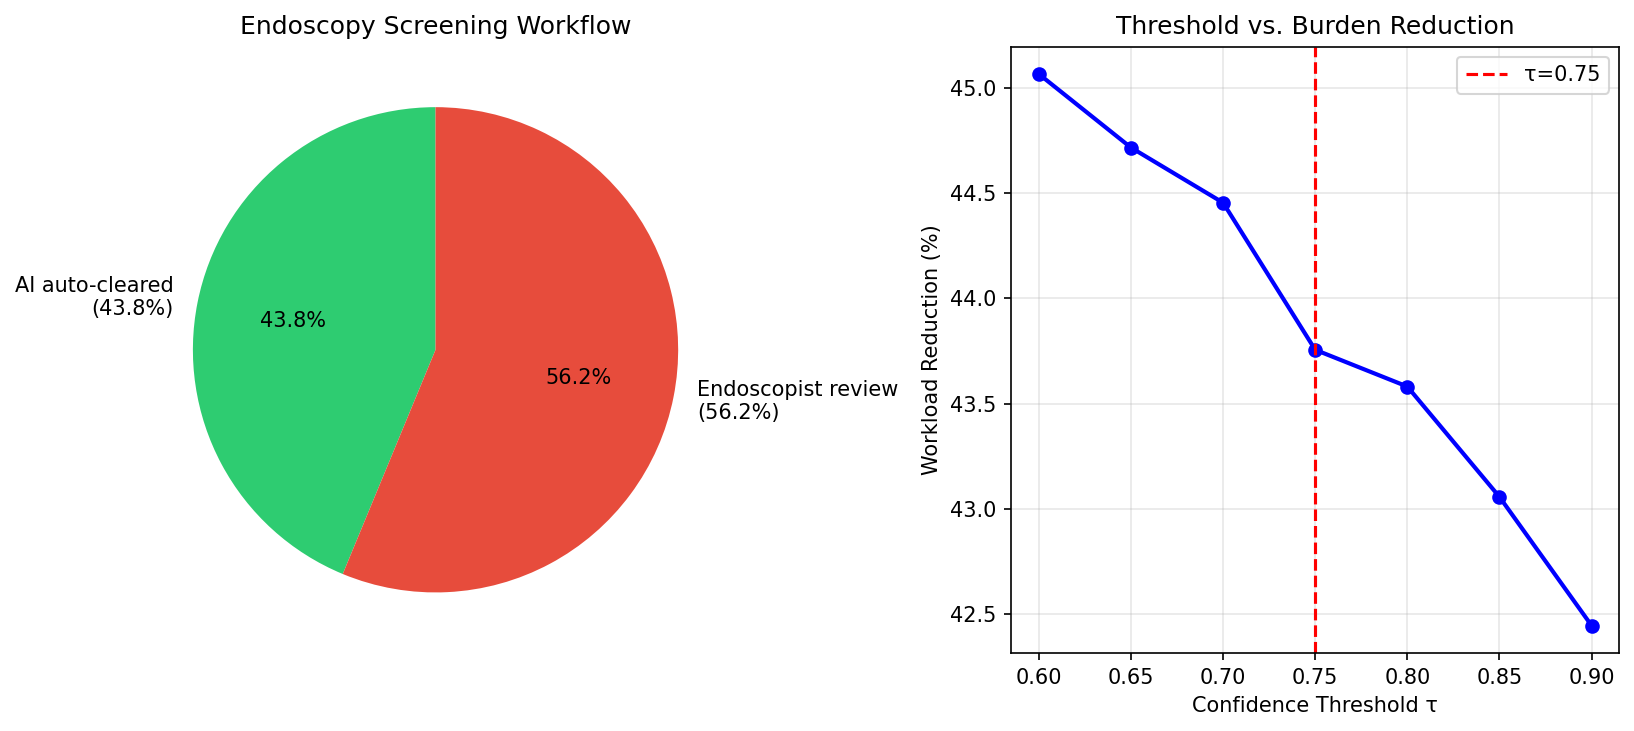
\includegraphics[width=\linewidth]{workload_simulation.png}
  \caption{Workload reduction (\%) and High-Risk escalation rate (\%)
    vs.\ MC Dropout threshold $\tau$ (best model, $T=30$ passes).
    $\tau=0.75$ is marked; all High-Risk cases escalated regardless
    of confidence.}
  \label{fig:workload}
\end{figure}

\subsection{GradCAM Explainability}

Figure~\ref{fig:gradcam} shows representative GradCAM heatmaps for one image
per risk class across all three architectures. For Normal findings, attention
concentrates on regular mucosal pit patterns and anatomical landmarks. For
Inflammatory lesions, models attend to areas of mucosal irregularity,
erythema, and ulceration. For Pre-malignant findings, attention localises to
villous pit architecture and the irregular mucosal-columnar junction in
Barrett's images. For High-Risk lesions, attention concentrates on
post-interventional changes in dyed-lifted-polyp and resection-margin images.
CNN architectures produce sharper, more spatially localized heatmaps, while
DeiT-Tiny shows broader patch-level attention patterns capturing global
mucosal context.

\begin{figure}[H]
  \centering
  \begin{subfigure}[b]{0.48\textwidth}
    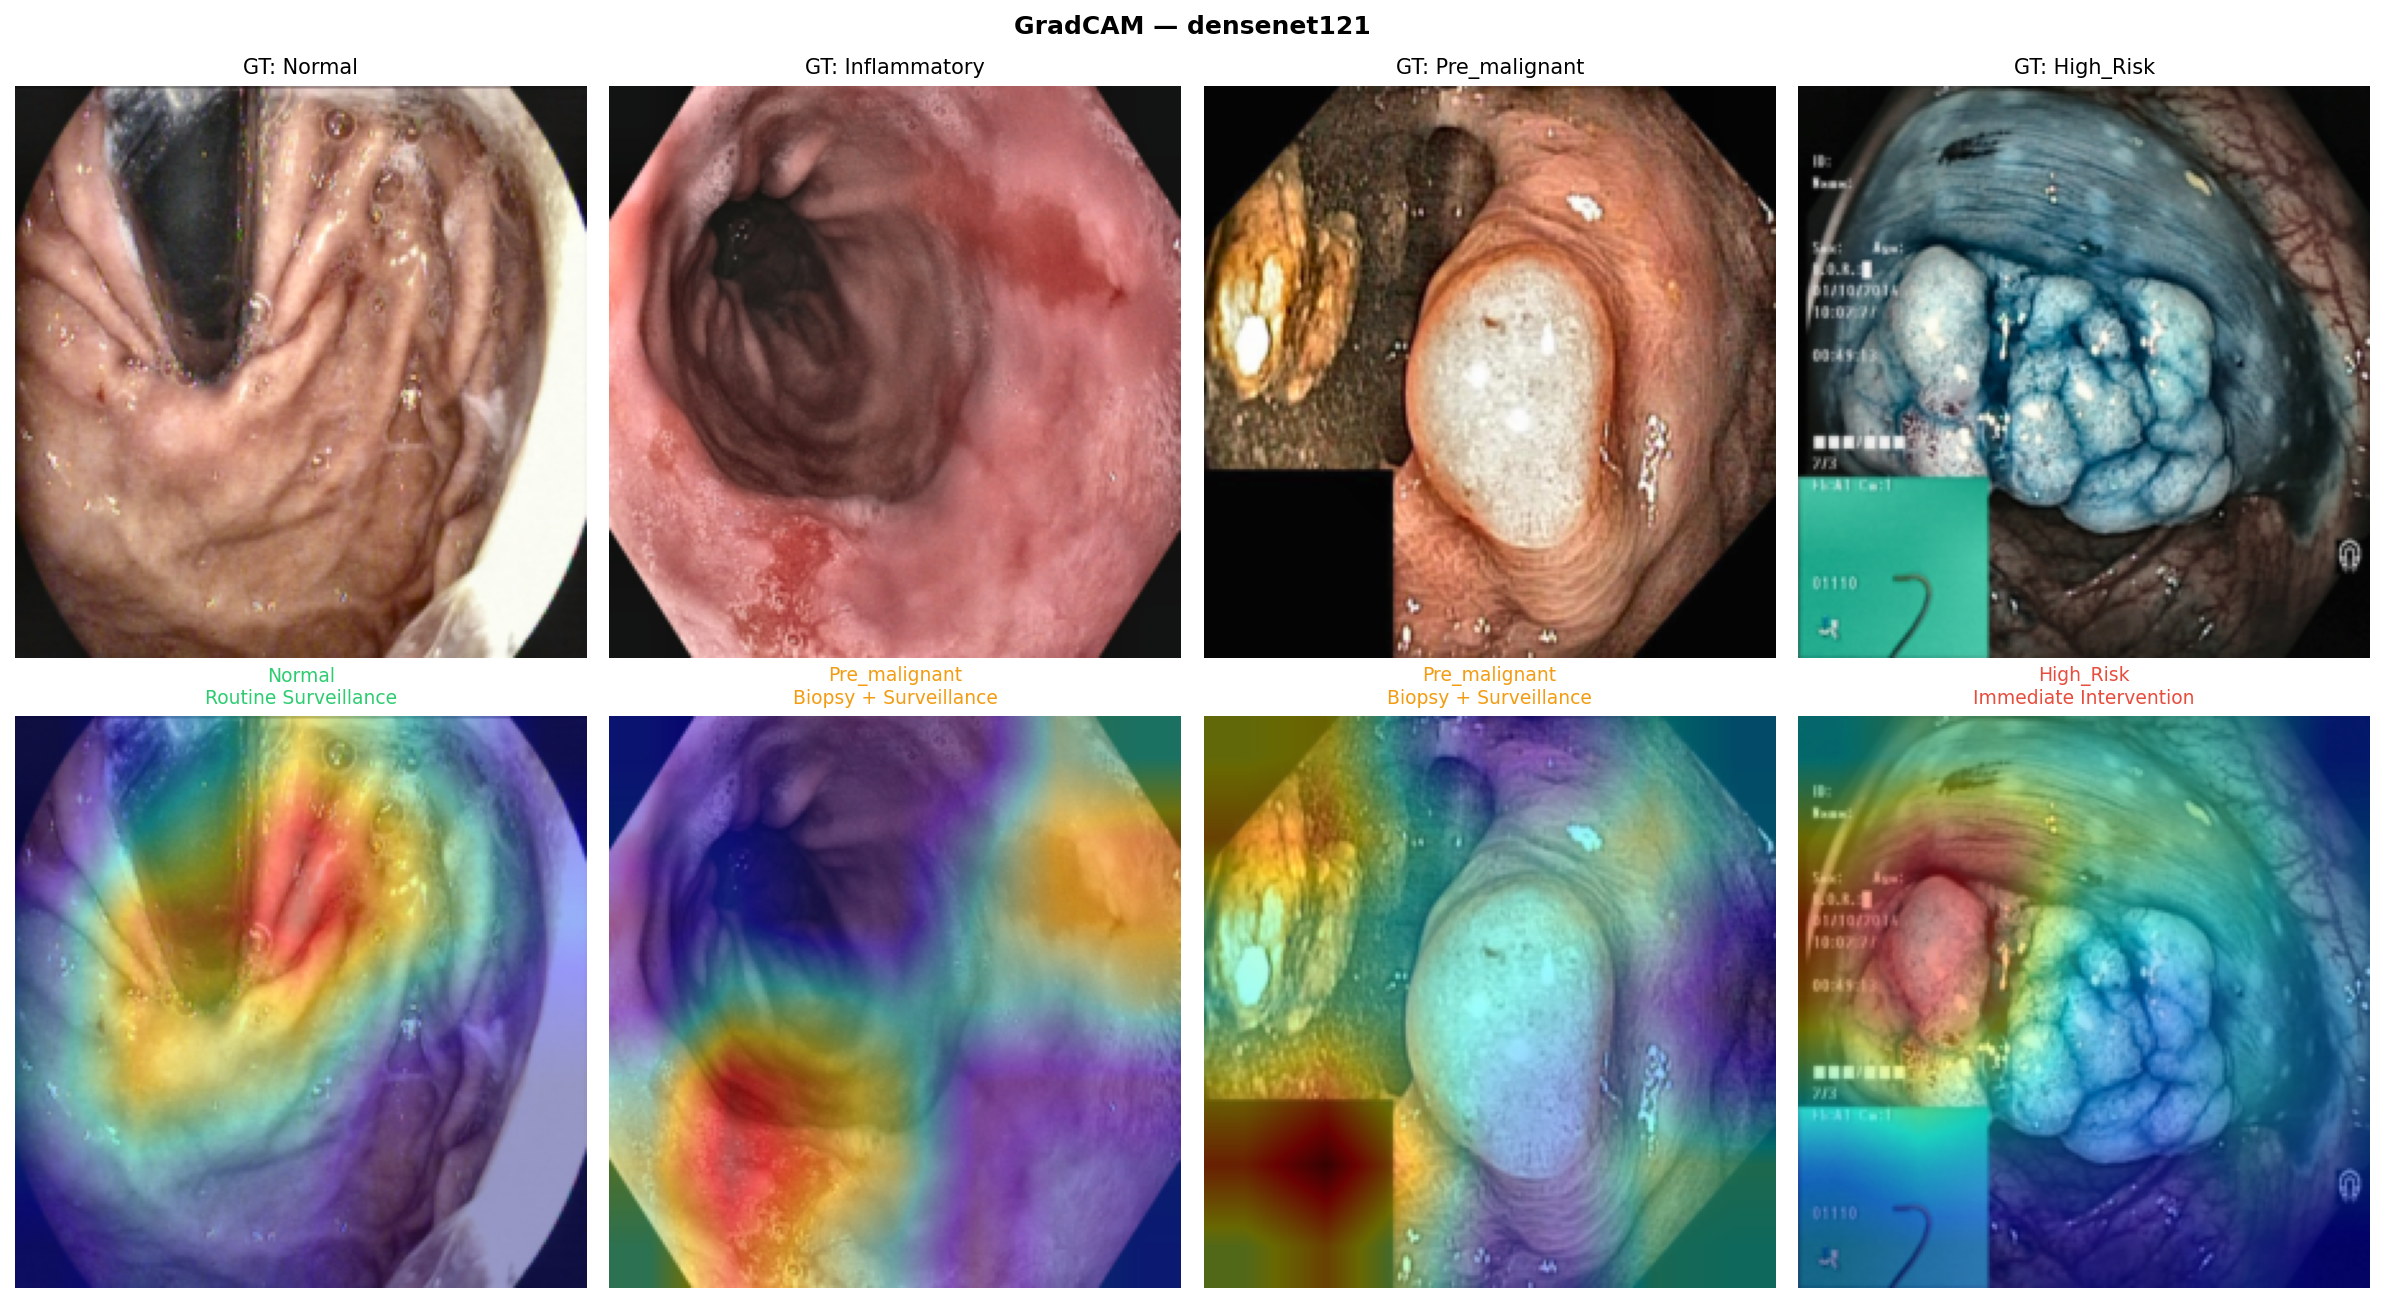
\includegraphics[width=\linewidth]{gradcam_densenet121.png}
    \caption{DenseNet-121}
  \end{subfigure}
  \hfill
  \begin{subfigure}[b]{0.48\textwidth}
    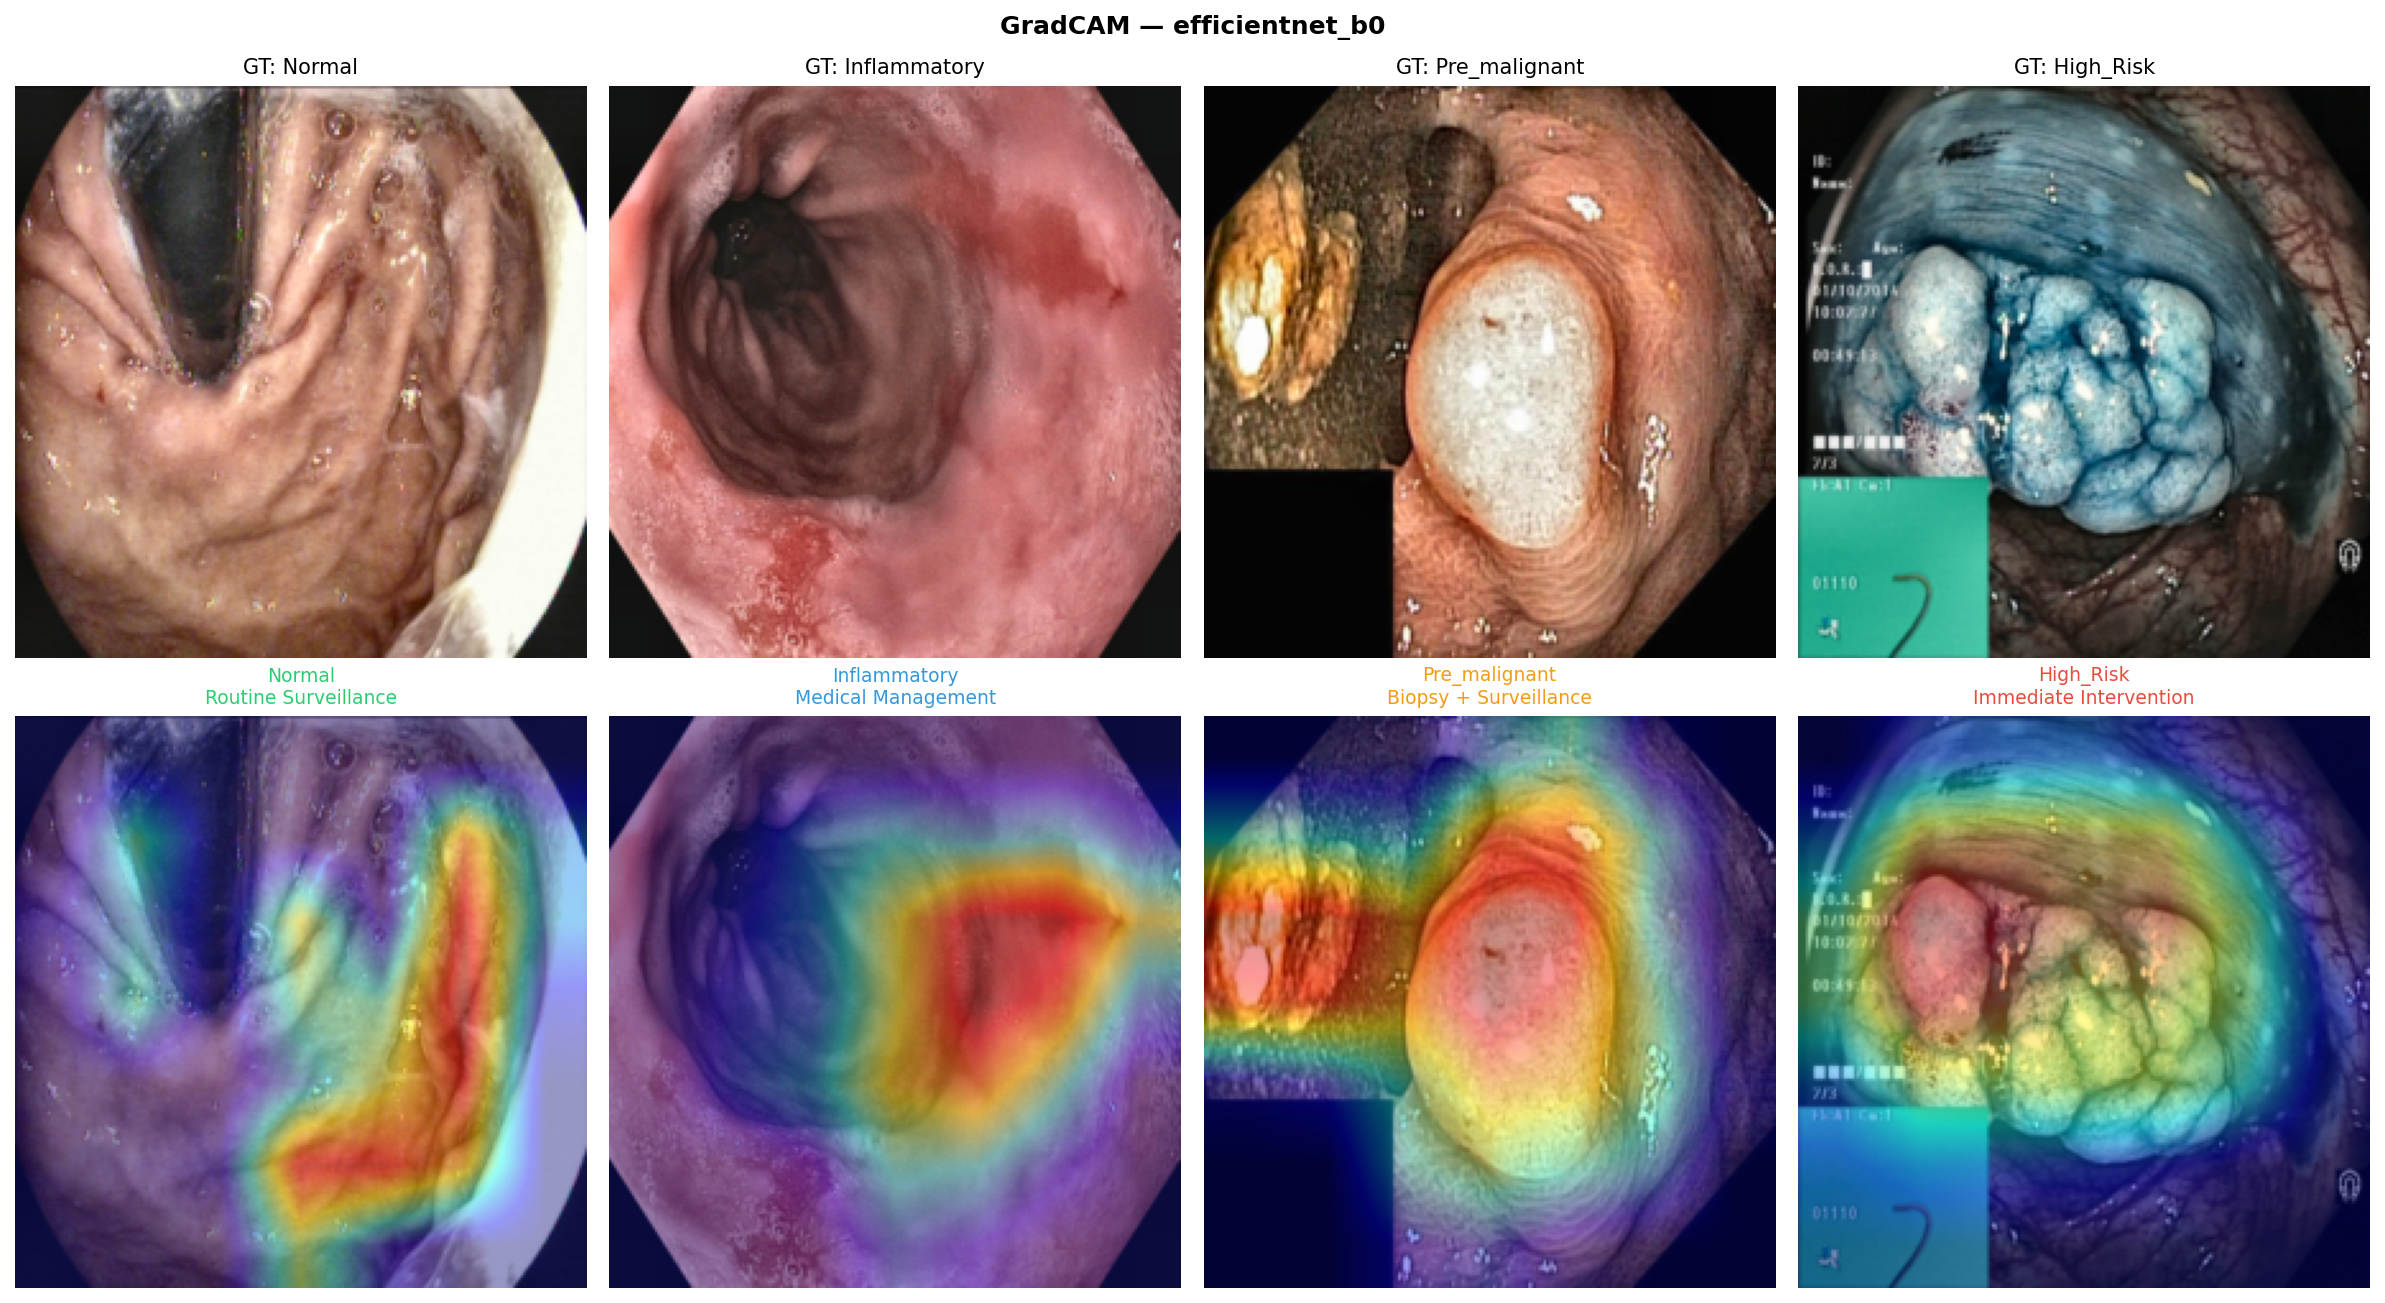
\includegraphics[width=\linewidth]{gradcam_efficientnet_b0.png}
    \caption{EfficientNet-B0}
  \end{subfigure}
  \par\vspace{4pt}
  \begin{subfigure}[b]{0.48\textwidth}
    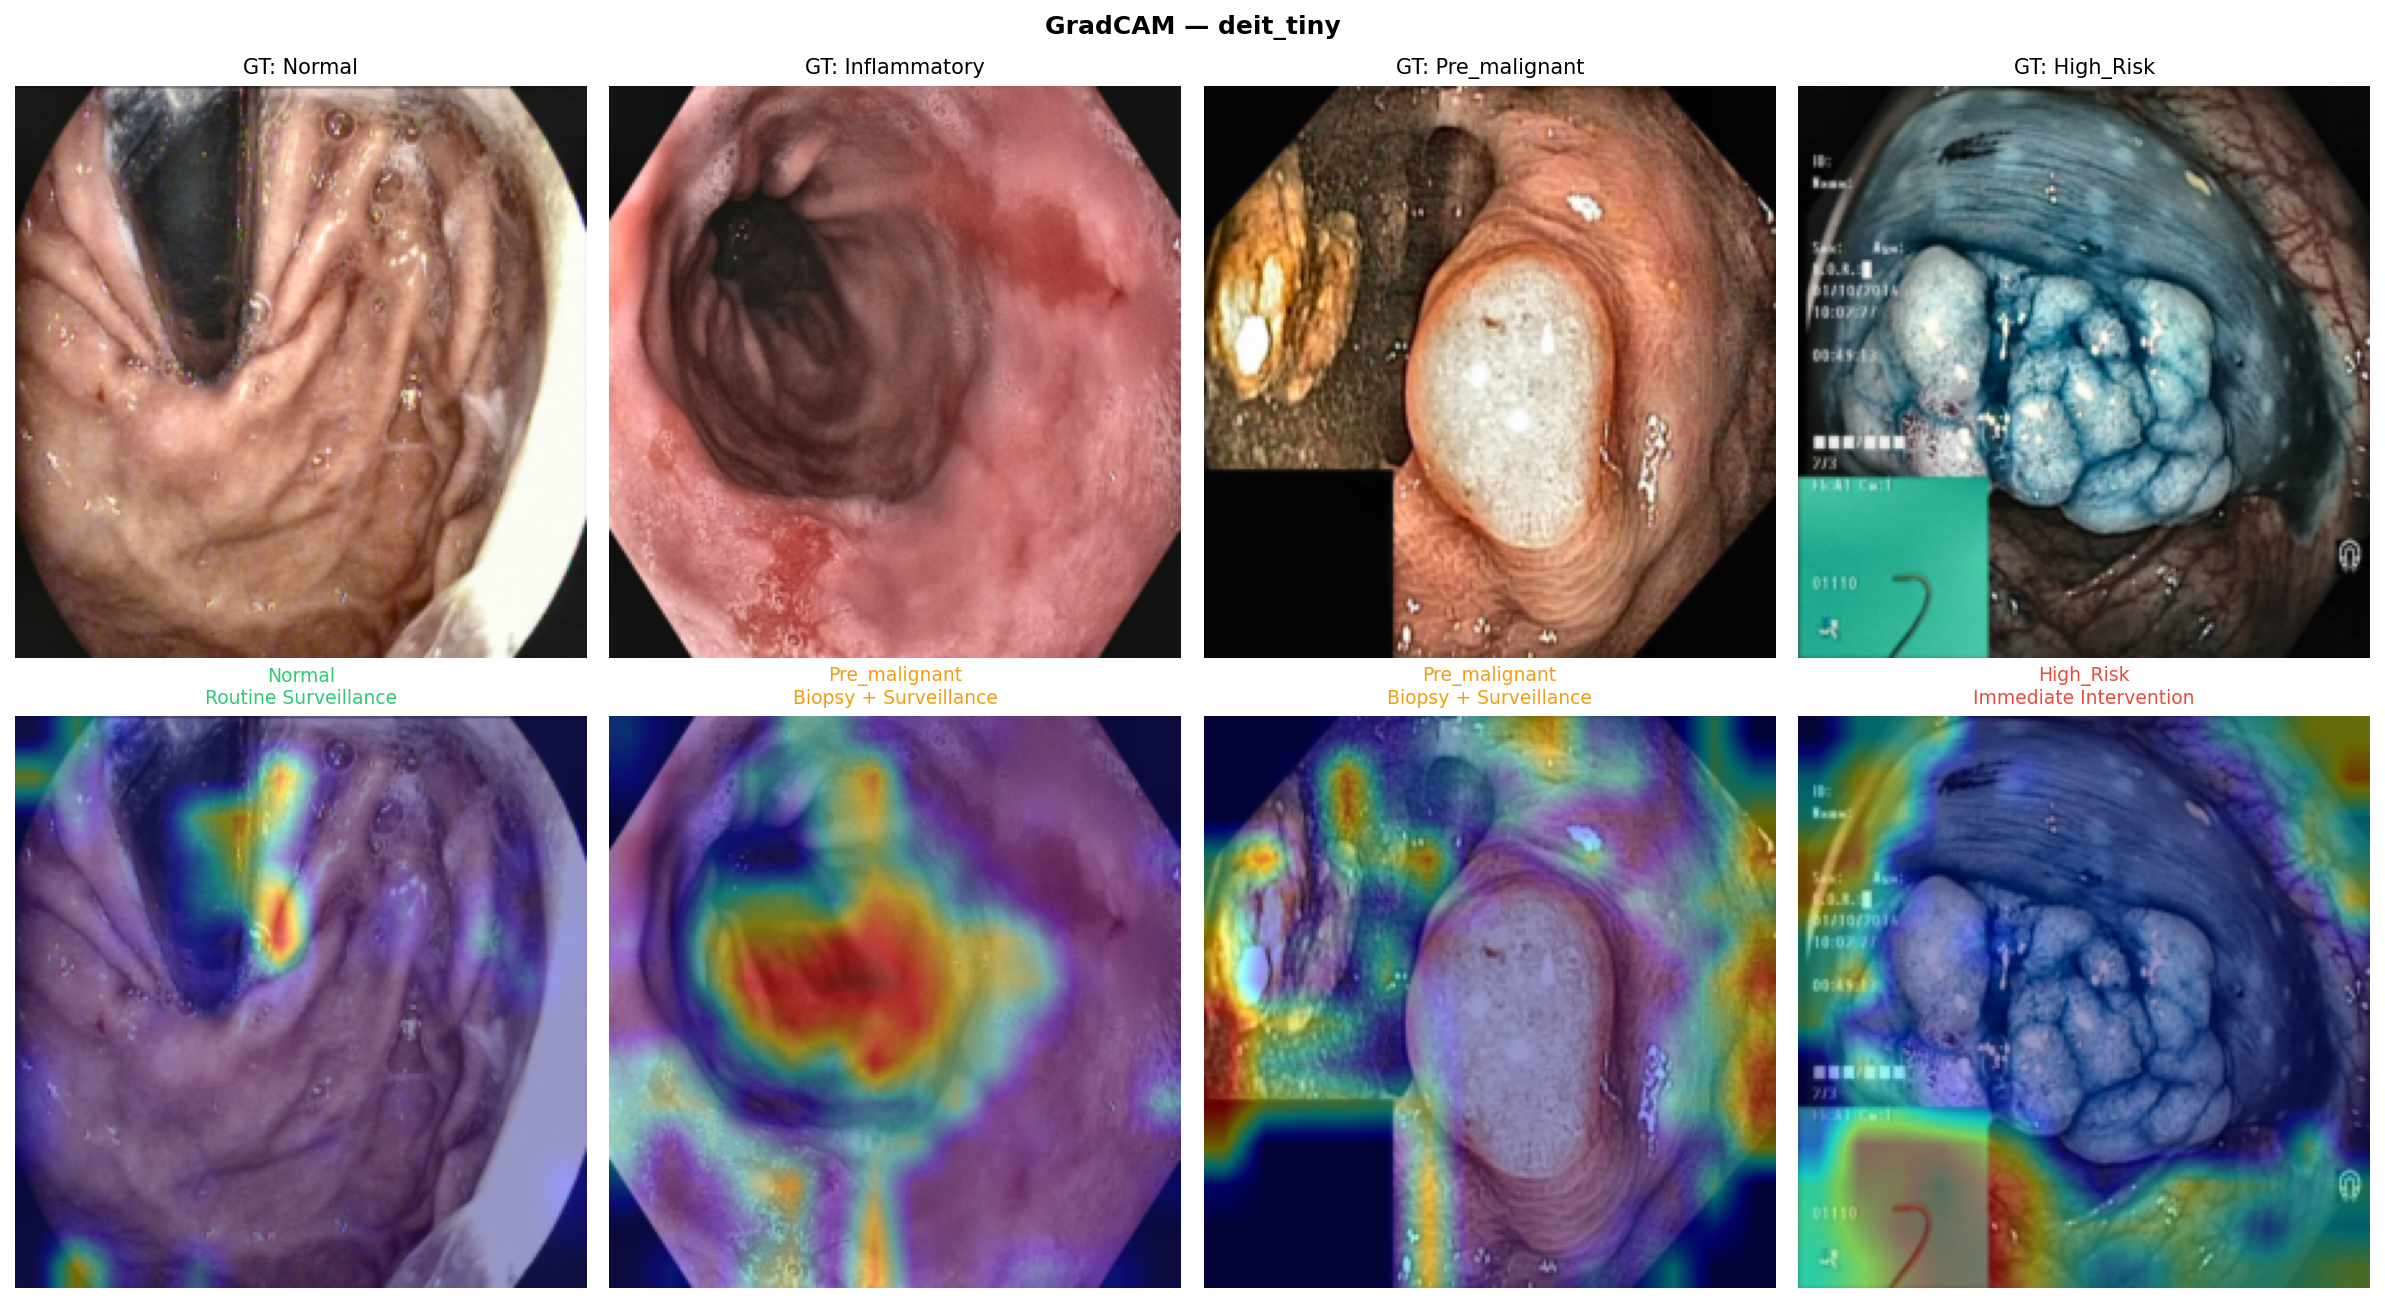
\includegraphics[width=\linewidth]{gradcam_deit_tiny.png}
    \caption{DeiT-Tiny}
  \end{subfigure}
  \caption{GradCAM heatmaps across four risk classes (Normal, Inflammatory,
    Pre-malignant, High-Risk) for all three architectures. Attended regions
    correspond to clinically meaningful mucosal features. CNN architectures
    produce sharper, spatially localized attention; DeiT-Tiny shows broader
    patch-level patterns capturing global mucosal context.}
  \label{fig:gradcam}
\end{figure}

\subsection{ROC Curves and Confusion Matrices}

Figure~\ref{fig:roc} shows one-vs-rest ROC-AUC curves per class for all
three models. Figure~\ref{fig:cm} shows normalized confusion matrices on the
HyperKvasir test set.

\begin{figure}[H]
  \centering
  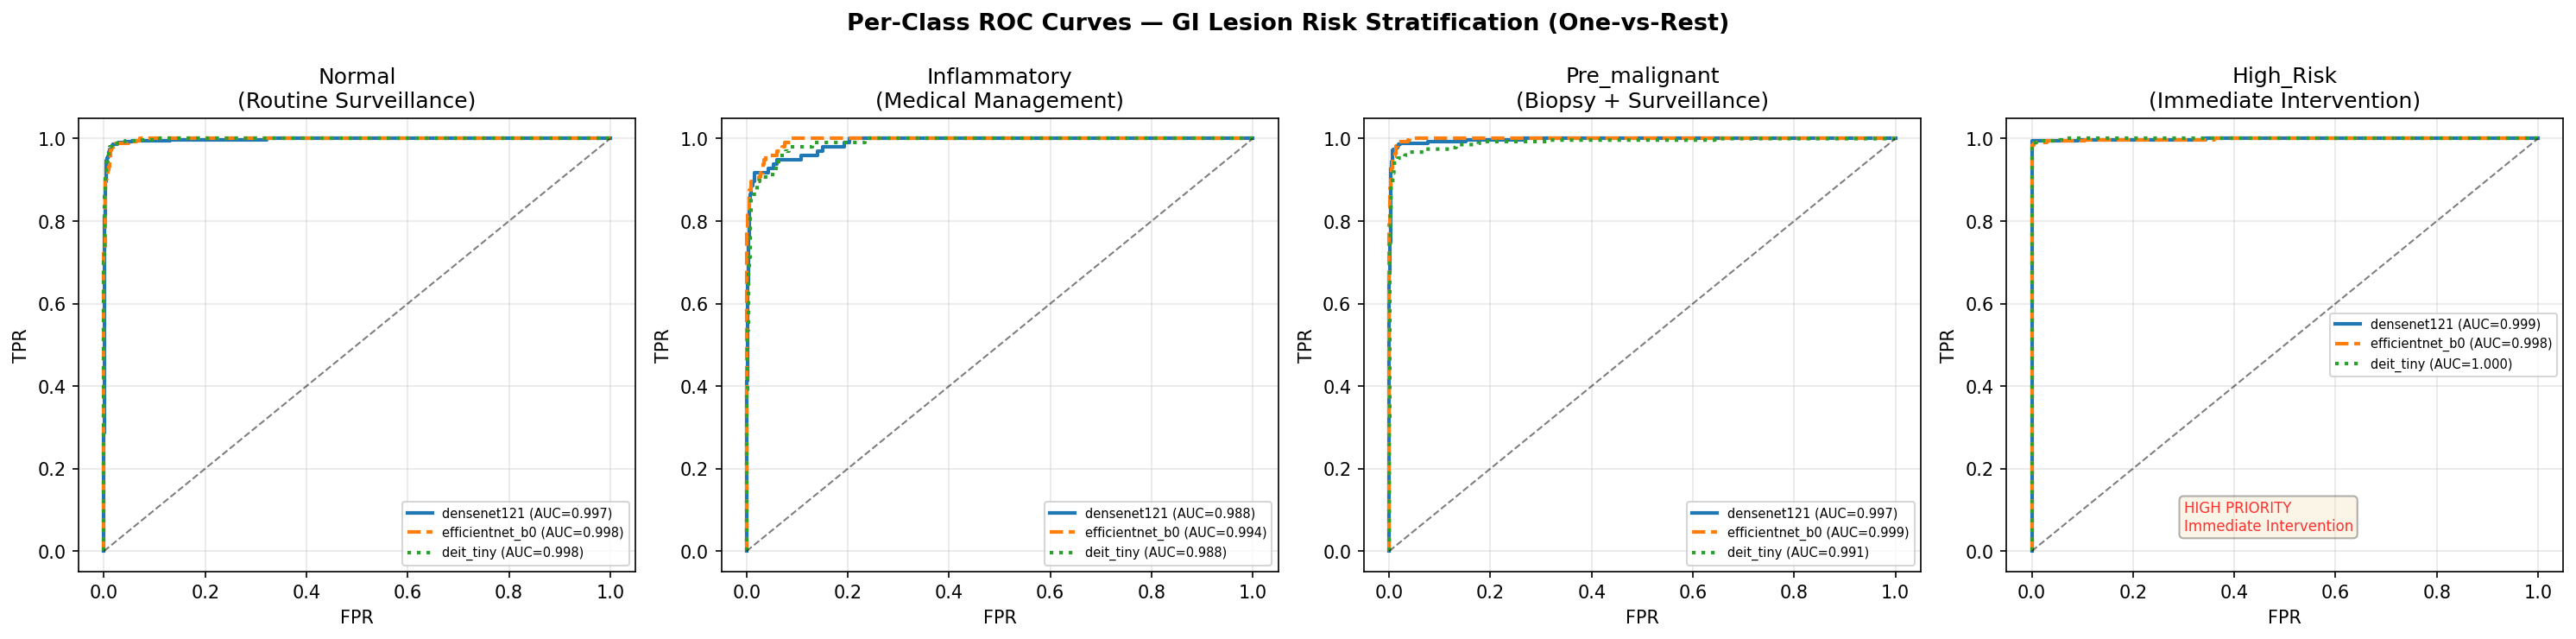
\includegraphics[width=0.80\textwidth]{roc_curves.png}
  \caption{One-vs-rest ROC-AUC curves per risk class for all three models
    on the HyperKvasir test set.}
  \label{fig:roc}
\end{figure}

\begin{figure}[H]
  \centering
  \begin{subfigure}[b]{0.32\textwidth}
    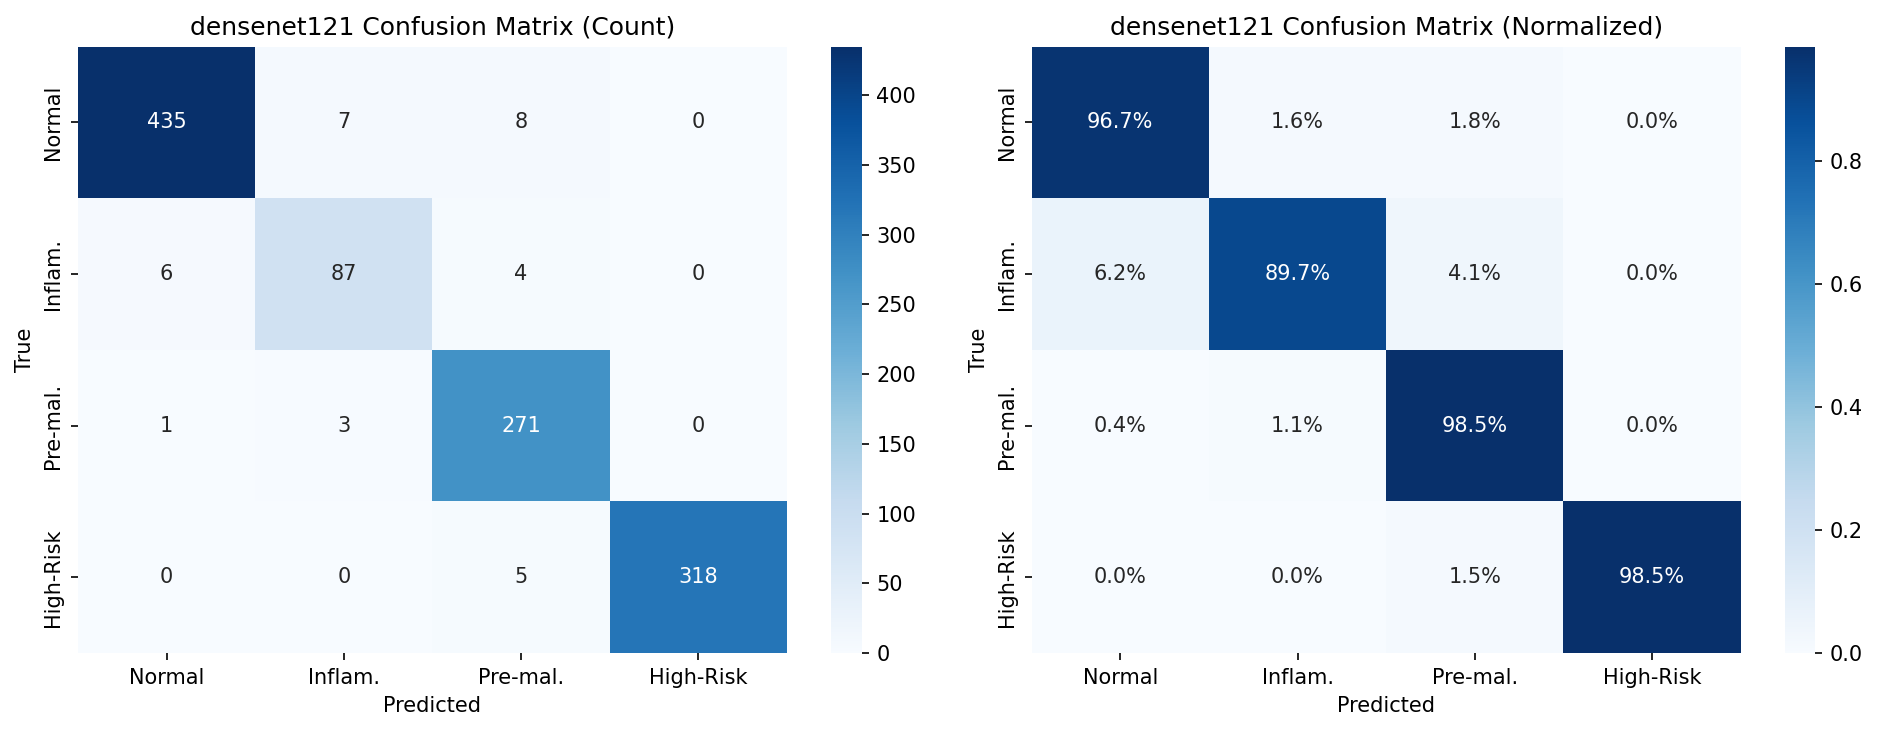
\includegraphics[width=\linewidth]{confusion_matrix_densenet121.png}
    \caption{DenseNet-121}
  \end{subfigure}
  \hfill
  \begin{subfigure}[b]{0.32\textwidth}
    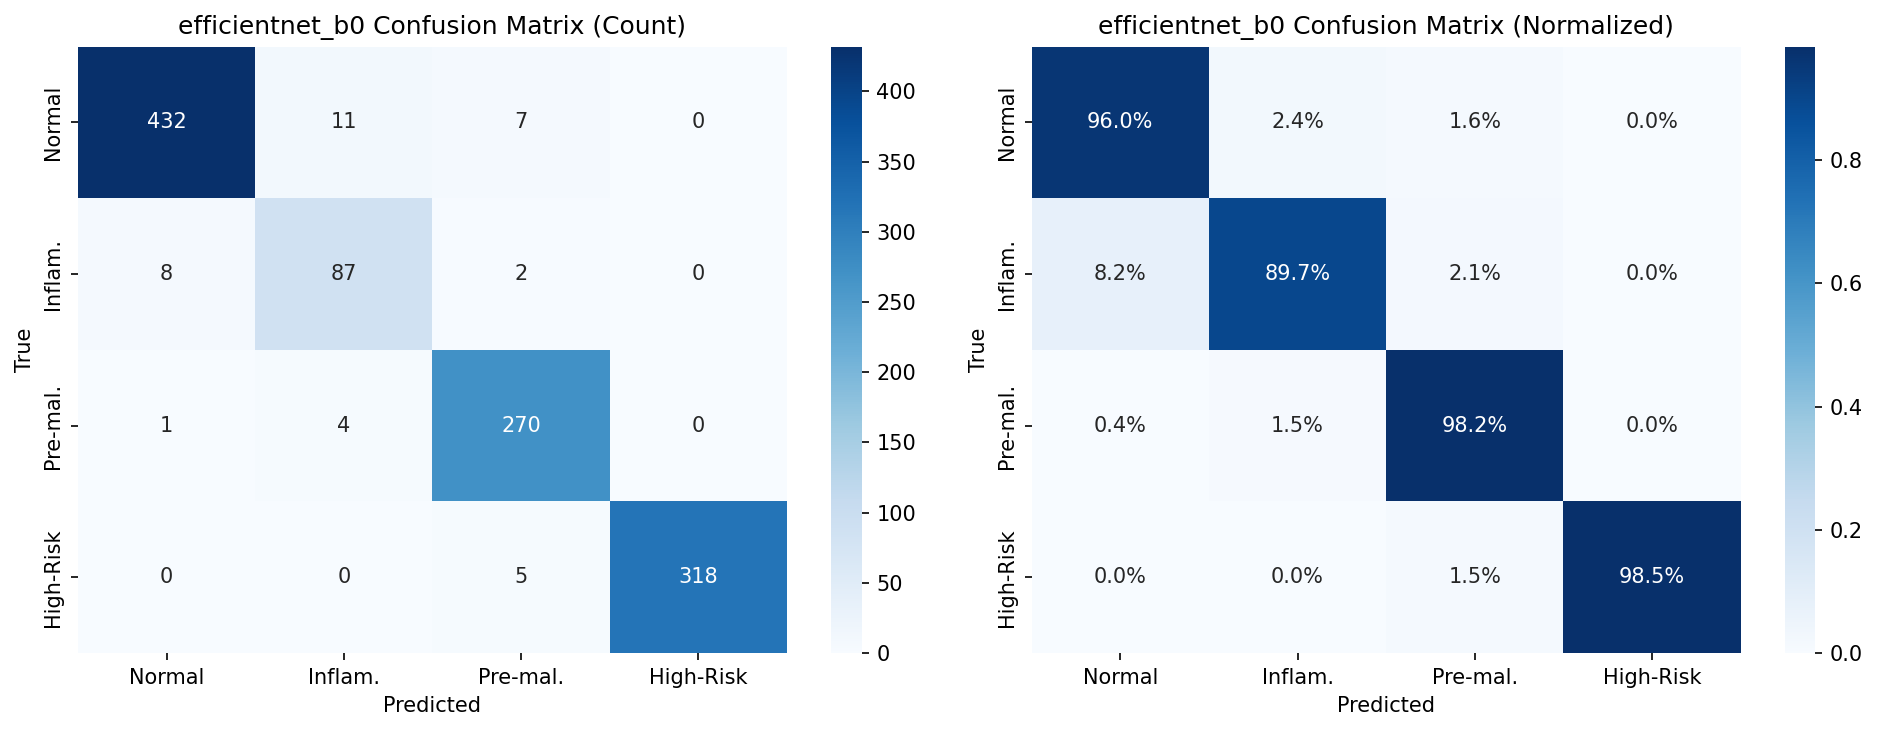
\includegraphics[width=\linewidth]{confusion_matrix_efficientnet_b0.png}
    \caption{EfficientNet-B0}
  \end{subfigure}
  \hfill
  \begin{subfigure}[b]{0.32\textwidth}
    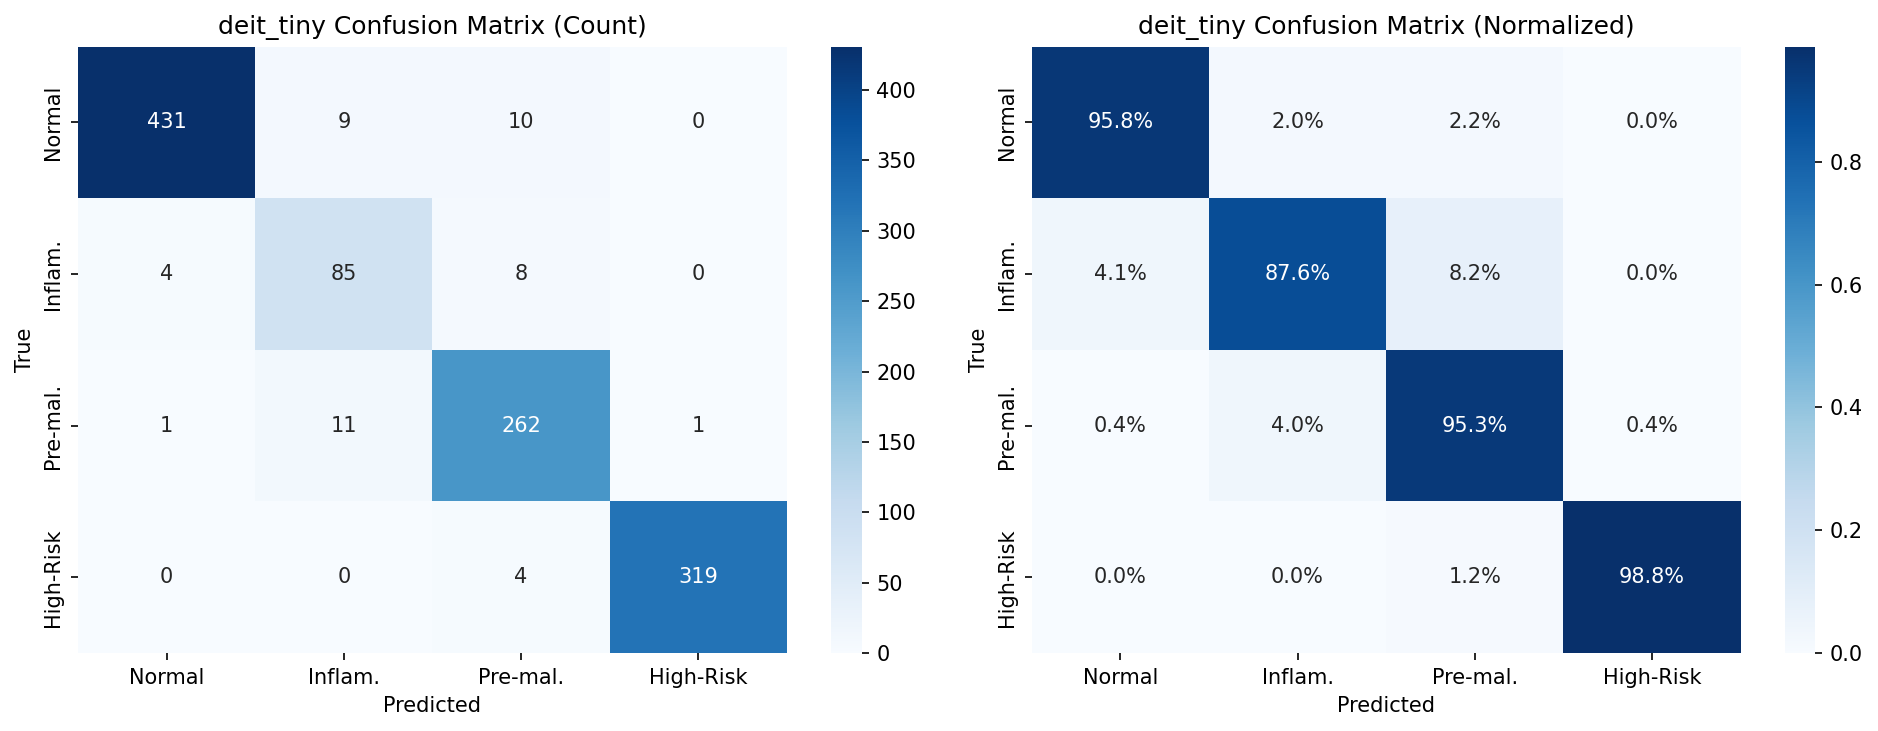
\includegraphics[width=\linewidth]{confusion_matrix_deit_tiny.png}
    \caption{DeiT-Tiny}
  \end{subfigure}
  \caption{Normalized confusion matrices on the HyperKvasir test set.
    Rows represent true labels; columns represent predicted labels.}
  \label{fig:cm}
\end{figure}

\subsection{Confusion Pattern Analysis}

The normalized confusion matrices (Figure~\ref{fig:cm}) reveal a consistent
error structure across all three architectures. The dominant misclassification
is Inflammatory predicted as Normal: EfficientNet-B0 achieves only 49\,\%
Inflammatory recall (Table~\ref{tab:per_class}), meaning more than half of
Inflammatory lesions are missed by the classifier. This is clinically
attributable to the visual overlap between grade-A esophagitis and normal
mucosa under the Los Angeles classification, compounded by the small class
size (97 test samples). The Pre-malignant tier is over-detected relative to
ground truth (precision\,=\,0.80 vs.\ recall\,=\,0.91), indicating a modest
tendency to upgrade Inflammatory findings to the Pre-malignant tier---a
conservative error that leads to unnecessary biopsy referral rather than
a missed lesion. High-Risk is strongly separated across all models
(precision\,=\,0.99, recall\,=\,0.95 for EfficientNet-B0), consistent
with the visually distinctive dye-staining patterns in the dyed-lifted-polyp
and resection-margin classes that dominate this tier. Critically, the
Inflammatory-to-Normal confusion does not produce a safety failure: an
Inflammatory lesion misclassified as Normal remains at tier~1 (medical
management needed), which MC Dropout does not escalate but which also does
not carry the mortality cost of a missed High-Risk lesion.

%% ============================================================================
\section{Discussion}
\label{sec:discussion}
%% ============================================================================

The benchmark results confirm the core premise: this form of
ACG/ESGE-aligned clinical risk tiering is achievable at under 8\,M
parameters, within the footprint of standard clinical endoscopy hardware.
EfficientNet-B0 led on macro F1 both in-domain (0.8319) and zero-shot
(0.7645 on Kvasir-v2), while DenseNet-121 produced the highest mean
AUC-ROC (0.9754). All three architectures achieved High-Risk recall
$\geq$\,94.4\,\% under direct classification and zero missed High-Risk
lesions under the MC Dropout referral protocol (the two figures are
consistent because of the Pre-malignant escalation mechanism described
in Section~\ref{sec:workload}).
The 5$\times$ High-Risk penalty reliably shifted each model toward
aggressive recall on the most critical class; macro F1 held within
a 0.02 band across all three architectures.

Comparing CNN and Transformer architectures under an identical parameter
budget ($<$8\,M) isolates inductive bias rather than capacity. DenseNet-121
and EfficientNet-B0 both exploit translation invariance and hierarchical
local feature extraction, which suits mucosal texture analysis well---pit
pattern irregularity and vascular architecture are spatially compact cues.
DeiT-Tiny, by contrast, processes the image as 196 non-overlapping patch
tokens and attends globally; this may benefit lesions whose diagnosis depends
on their spatial context, such as the completeness of dyed resection margins.
In practice the performance gap between CNN and Transformer was narrow
(0.8319 vs.\ 0.8134 macro F1), suggesting that for this resolution and
dataset size, local texture remains the dominant discriminative signal.

Inspecting the GradCAM heatmaps, none of the three models appeared to latch
onto endoscope shaft reflections, text overlays, or other image artifacts.
CNN heatmaps were tighter and more focal---consistent with the local
receptive fields of convolutional filters---while DeiT-Tiny produced
broader, patch-spanning activations. For High-Risk cases, both CNN models
concentrated attention on the dye boundary in lifted-polyp images, which
aligns with how endoscopists visually assess resection completeness. Whether
the broader DeiT attention represents richer contextual reasoning or simply
lower spatial resolution in the token grid warrants further study with
higher-resolution Transformer variants.

Zero-shot performance on Kvasir-v2 dropped markedly for DenseNet-121
(0.8270\,→\,0.6415) but much less for EfficientNet-B0 (0.8319\,→\,0.7645)
and DeiT-Tiny (0.8134\,→\,0.7603). The larger DenseNet drop likely reflects
overfitting to HyperKvasir's specific color balance and artifact
distribution; its Normal class recall fell to 55\,\% on Kvasir-v2 compared
with 94\,\% in-domain. CLAHE preprocessing normalizes local contrast and
appears to assist EfficientNet-B0 and DeiT-Tiny but cannot eliminate
sensor-level domain shift. Multi-source training and feature-level domain
adaptation are natural next steps.

\subsection{Inflammatory Class Performance}

Inflammatory lesions yielded the lowest per-class F1 across all three
architectures, attributable to two compounding factors. First, the
Inflammatory tier has the smallest class representation in HyperKvasir
(645 images vs.\ 1,836--3,000 for other tiers), limiting the diversity of
training examples even under WeightedRandomSampler. Second, mild inflammatory
findings---particularly early \texttt{esophagitis-a} and \texttt{hemorrhoids}
---share mucosal texture characteristics with both normal mucosa and low-grade
pre-malignant findings, creating inherent visual ambiguity at class boundaries.
Human endoscopists face the same ambiguity: grade-A esophagitis under the
Los Angeles classification is frequently confused with normal mucosa even
by experienced observers. The model's difficulty on this tier reflects a
genuinely hard visual boundary, not a correctable architectural weakness. This class-level weakness does not translate into a safety failure,
however: an Inflammatory lesion misclassified as Normal results in
delayed medical management rather than a missed resection---a
qualitatively less severe outcome than a missed High-Risk lesion. This asymmetry is precisely what the
AEL encodes, and High-Risk recall remained above 94\,\% across all
architectures regardless of Inflammatory class performance.

\subsection{Clinical Workload Impact}

The 43.8\,\% workload reduction translates directly into endoscopist time.
A high-volume GI unit reviewing 60 cases per session would have approximately
26 cases auto-cleared by the AI triage layer, leaving 34 for endoscopist
review. Assuming an average review time of 3--5 minutes per flagged case,
this represents a saving of 78--130 minutes per session---equivalent to
reclaiming one to two additional procedure slots per list. The safety
guarantee is structural: the MC Dropout referral protocol escalates every
Pre-malignant and High-Risk prediction regardless of model confidence, so
workload reduction is achieved exclusively by clearing high-confidence Normal
and Inflammatory cases, the two tiers where a miss carries the lowest clinical
consequence. The 501 auto-cleared cases in the test set contained zero
High-Risk lesions (Table~\ref{tab:workload}), confirming that the safety
constraint holds empirically in addition to being guaranteed by design.
Deployment impact would depend on the local prevalence of high-risk findings:
in a high-prevalence tertiary referral population the auto-clearance rate
would fall, but the safety guarantee would remain unchanged.

\subsection{Limitations}

Several limitations should be acknowledged. \emph{First}, HyperKvasir was
collected at a single institution (Baerum Hospital, Norway) using a limited
range of endoscopy systems; performance in multi-site deployments remains to
be evaluated. \emph{Second}, the four-class risk schema, while grounded in
ACG/ESGE guidelines, represents a simplification: clinical practice involves
nuanced intra-class variation (e.g., polyp histology) that cannot be
determined from optical endoscopy alone. \emph{Third}, MC Dropout with $T=30$ passes
provides an approximation to Bayesian posterior inference that may
underestimate calibration uncertainty compared to ensemble methods.
Reliability diagrams and Expected Calibration Error (ECE) were evaluated
on the held-out test set: DenseNet-121 achieves ECE\,=\,0.0149,
EfficientNet-B0 ECE\,=\,0.0259, and DeiT-Tiny ECE\,=\,0.0314, indicating
well-calibrated confidence estimates across all three architectures
(ECE\,$<$\,0.05 is the conventional threshold for good calibration).
Nonetheless, post-hoc recalibration via temperature scaling and evaluation
on an independent prospective cohort should precede clinical deployment.
\emph{Fourth}, a single stratified 70/15/15 split (seed\,=\,42) is used
throughout; a $k$-fold evaluation would provide tighter estimates of
split-to-split variance on HyperKvasir. The zero-shot Kvasir-v2
evaluation partially substitutes for this by testing generalization
on a completely independent cohort. \emph{Fifth}, all experiments ran on Apple M2 MPS hardware. Parameter
count is a useful proxy for model size but does not translate directly
to inference latency: memory bandwidth, operator support, and quantization
efficiency all differ substantially across MPS, embedded GPUs, and the
dedicated accelerators in clinical endoscopy towers. On the M2 device
used here, DenseNet-121 averaged 14\,ms per image (median 13.6\,ms,
$\approx$71\,fps); this is an indicative figure only, and frame-rate
characterization on representative clinical hardware (e.g., NVIDIA
Quadro or embedded FPGA accelerators) should precede any real-time
deployment claim.

%% ============================================================================
\section{Conclusions}
\label{sec:conclusions}
%% ============================================================================

Across three architectures and two datasets, the case for lightweight
guideline-aligned risk stratification is clear: sub-8\,M parameter
models can replicate the four-tier ACG/ESGE clinical schema without
purpose-built hardware. EfficientNet-B0 achieves macro
F1\,=\,0.8319 in-domain and 0.7645 zero-shot on Kvasir-v2; all three
architectures reach zero missed High-Risk lesions under MC Dropout
referral, with 43.8\,\% of cases auto-cleared (high-confidence Normal and Inflammatory
predictions)---reducing endoscopist review burden without
compromising safety. DenseNet-121 leads on mean AUC-ROC (0.9754),
and GradCAM confirms that model attention concentrates on mucosal
features a clinician would recognize rather than imaging artifacts.

The 5$\times$ High-Risk penalty in AEL maintained $\geq$94\,\%
High-Risk recall across all three architectures even when the Inflammatory class
remained difficult (F1\,=\,0.57 for EfficientNet-B0), confirming that
survival-cost asymmetry can be encoded directly into the training objective
without sacrificing overall macro performance. The MC Dropout referral protocol
converts a probabilistic classifier into a structurally safe screening tool by
escalating all Pre-malignant and High-Risk predictions regardless of
confidence---a safety property achievable on existing endoscopy hardware without
retraining.

Several open questions remain for future work. Multi-site validation is the most
pressing: the DenseNet-121 zero-shot drop from 0.8270 to 0.6415
(Table~\ref{tab:xdataset}) illustrates the sensor-level domain shift that
multi-source training must address before clinical deployability can be
established. Extending the four-class schema to incorporate polyp morphology
(Paris classification) and optical biopsy predictions would align the model
output more precisely with the clinical decision chain, particularly for the
Pre-malignant tier. Finally, foundation model feature extractors combined with
multiple instance learning over full procedure frame sequences offer a path
toward continuous risk surveillance across an entire endoscopy session, with
domain adaptation strategies addressing the cross-institutional color and sensor
shift documented in the DenseNet-121 zero-shot results.

%% ============================================================================
\section*{Declarations}

\noindent\textbf{Ethics approval}\quad This study used only publicly
available, fully anonymized datasets (HyperKvasir and Kvasir-v2). No
human subjects were recruited and no patient-identifiable data were
accessed. Institutional ethics approval was therefore not required.

\noindent\textbf{Author contributions}\quad
Azizur Rahman: Conceptualization, Methodology, Software, Formal analysis,
Investigation, Data curation, Visualization, Writing -- original draft.
Nakib Uddin Ahmed: Software, Validation, Writing -- review \& editing.
Mehjabin Ferdous: Clinical guideline validation, Resources,
Writing -- review \& editing.
Kadirur Rahman Chowdhury: Conceptualization, Supervision,
Writing -- review \& editing.

\noindent\textbf{Funding}\quad The authors received no specific funding
for this work.

\noindent\textbf{Conflict of interest}\quad The authors declare no
competing interests.

\noindent\textbf{Data availability}\quad HyperKvasir and Kvasir-v2 are
publicly available datasets. Code and trained model checkpoints will be
released upon acceptance.

%% ============================================================================
\subsection*{Author Biographies}

\noindent\textbf{Azizur Rahman} is a researcher at Indiana Wesleyan University
and RadTH Technologies. His work focuses on medical image analysis, clinical AI
systems, and deep learning for healthcare.

\noindent\textbf{Nakib Uddin Ahmed} is a software engineer and ML practitioner.
His research interests include computer vision and validation of AI-assisted
diagnostic systems.

\noindent\textbf{Mehjabin Ferdous} (MPH, St.\ Francis College) is a public
health professional specializing in clinical guideline review and healthcare
resource management.

\noindent\textbf{Kadirur Rahman Chowdhury} is a researcher and academic
supervisor with expertise in biomedical engineering and AI-driven clinical
decision support.

%% ============================================================================

\begin{thebibliography}{99}

\bibitem[Sung et~al.(2021)]{Sung2021}
Sung H, Ferlay J, Siegel RL, et~al.
\newblock Global cancer statistics 2020: {GLOBOCAN} estimates of incidence and
  mortality worldwide for 36 cancers in 185 countries.
\newblock \emph{CA Cancer J Clin}. 2021;71(3):209--249.

\bibitem[Kaminski et~al.(2017)]{Kaminski2017}
Kaminski MF, Thomas-Gibson S, Bugajski M, et~al.
\newblock Performance measures for lower gastrointestinal endoscopy: a
  {European Society of Gastrointestinal Endoscopy (ESGE)} quality improvement
  initiative.
\newblock \emph{Endoscopy}. 2017;49(4):378--397.

\bibitem[Wang et~al.(2019)]{Wang2019}
Wang P, Berzin TM, Glissen Brown JR, et~al.
\newblock Real-time automatic detection system increases colonoscopic polyp and
  adenoma detection rates: a prospective randomized controlled study.
\newblock \emph{Gut}. 2019;68(10):1813--1819.

\bibitem[Pogorelov et~al.(2017a)]{Pogorelov2017}
Pogorelov K, Randel KR, Griwodz C, et~al.
\newblock {KVASIR}: a multi-class image dataset for computer aided
  gastrointestinal disease detection.
\newblock In: \emph{Proceedings of the ACM MMSys}; 2017. p.~164--169.

\bibitem[Shaukat et~al.(2021)]{Shaukat2021}
Shaukat A, Kahi CJ, Burke CA, et~al.
\newblock {ACG} clinical guidelines: colorectal cancer screening 2021.
\newblock \emph{Am J Gastroenterol}. 2021;116(3):458--479.

\bibitem[Ferlitsch et~al.(2017)]{Ferlitsch2017}
Ferlitsch M, Moss A, Hassan C, et~al.
\newblock Colorectal polypectomy and endoscopic mucosal resection: {European
  Society of Gastrointestinal Endoscopy (ESGE)} clinical guideline.
\newblock \emph{Endoscopy}. 2017;49(3):270--297.

\bibitem[Rawla et~al.(2019)]{Rawla2019}
Rawla P, Sunkara T, Barsouk A.
\newblock Epidemiology of colorectal cancer: incidence, mortality, survival,
  and risk factors.
\newblock \emph{Gastroenterol Rev}. 2019;14(2):89--103.

\bibitem[Tajbakhsh et~al.(2016)]{Tajbakhsh2016}
Tajbakhsh N, Gurudu SR, Liang J.
\newblock Automated polyp detection in colonoscopy videos using shape and
  context information.
\newblock \emph{IEEE Trans Med Imaging}. 2016;35(2):630--644.

\bibitem[Ebigbo et~al.(2019)]{Ebigbo2019}
Ebigbo A, Mendel R, Probst A, et~al.
\newblock Computer-aided diagnosis using deep learning for the evaluation of
  malignant potential of gastric subepithelial lesions.
\newblock \emph{Sci Rep}. 2019;9(1):4465.

\bibitem[Dosovitskiy et~al.(2021)]{Dosovitskiy2021}
Dosovitskiy A, Beyer L, Kolesnikov A, et~al.
\newblock An image is worth $16\times16$ words: transformers for image
  recognition at scale.
\newblock In: \emph{International Conference on Learning Representations};
  2021.

\bibitem[Touvron et~al.(2021)]{Touvron2021}
Touvron H, Cord M, Douze M, et~al.
\newblock Training data-efficient image transformers and distillation through
  attention.
\newblock In: \emph{Proceedings of ICML}; 2021. p.~10347--10357.


\bibitem[Lin et~al.(2017)]{Lin2017}
Lin TY, Goyal P, Girshick R, et~al.
\newblock Focal loss for dense object detection.
\newblock In: \emph{Proceedings of ICCV}; 2017. p.~2980--2988.

\bibitem[Borgli et~al.(2020)]{Borgli2020}
Borgli H, Thambawita V, Smedsrud PH, et~al.
\newblock {HyperKvasir}, a comprehensive multi-class image and video dataset
  for gastrointestinal endoscopy.
\newblock \emph{Sci Data}. 2020;7(1):283.

\bibitem[Pogorelov et~al.(2017b)]{Pogorelov2017b}
Pogorelov K, Randel KR, Espeland T, et~al.
\newblock Kvasir: a multi-class image dataset for computer aided
  gastrointestinal disease detection.
\newblock In: \emph{Proceedings of the 8th ACM MMSys}; 2017.

\bibitem[Reza(2004)]{Reza2004}
Reza AM.
\newblock Realization of the contrast limited adaptive histogram equalization
  ({CLAHE}) for real-time image enhancement.
\newblock \emph{J VLSI Signal Process}. 2004;38(1):35--44.

\bibitem[Huang et~al.(2017)]{Huang2017}
Huang G, Liu Z, van~der Maaten L, Weinberger KQ.
\newblock Densely connected convolutional networks.
\newblock In: \emph{Proceedings of CVPR}; 2017. p.~4700--4708.

\bibitem[Tan \& Le(2019)]{Tan2019}
Tan M, Le QV.
\newblock {EfficientNet}: rethinking model scaling for convolutional neural
  networks.
\newblock In: \emph{Proceedings of ICML}; 2019. p.~6105--6114.

\bibitem[Selvaraju et~al.(2017)]{Selvaraju2017}
Selvaraju RR, Cogswell M, Das A, et~al.
\newblock {Grad-CAM}: visual explanations from deep networks via
  gradient-based localization.
\newblock In: \emph{Proceedings of ICCV}; 2017. p.~618--626.

\bibitem[Gal \& Ghahramani(2016)]{Gal2016}
Gal Y, Ghahramani Z.
\newblock Dropout as a {Bayesian} approximation: representing model uncertainty
  in deep learning.
\newblock In: \emph{Proceedings of ICML}; 2016. p.~1050--1059.

\end{thebibliography}

\end{document}
